% -----------------------------------------------
% Styl pro psaní diplomových a bakalářských prací
% -----------------------------------------------
\documentclass[a4paper,12pt]{book} % pro oboustranný tisk zvolte {book}!
% velikost stránky
\usepackage[tmargin=2cm,bmargin=2.5cm,rmargin=2cm,lmargin=3.5cm]{geometry}
% volba kódování, nastaveno je unicode
\usepackage[utf8]{inputenc}
% \usepackage[cp1250]{inputenc}
% \usepackage[latin2]{inputenc}
\usepackage[english]{babel}
%\def\refname{Literatura}
% pomocná makra pro sazbu matematických výrazů
\usepackage{amssymb} %na psaní dvojitých písem a zvlastních znaků (např. \varkappa)
\usepackage{amsmath}
% balíček pro vkládání obrázků
\usepackage{graphicx}
\usepackage{subfig}
% balíček pro obrázky na krajích stránky 
%\usepackage{floatflt}
% balíček pro křížové odkazy
\usepackage[unicode,bookmarksopen,colorlinks=false,plainpages=false,urlcolor=blue,pdfpagelabels]{hyperref}
% balíček pro vkládání hypertextových odkazů
\usepackage{url}

\usepackage{float}
\usepackage{lastpage}

%\usepackage[numbers]{natbib}

\usepackage[
backend=biber,
style=iso-numeric,
sorting=none
]{biblatex}
\addbibresource{citations.bib}

%style=phys,

%
% -----------------------------------------------
% Přepínač mezi bakalářskou a diplomovou prací, 
% barevným a černobílým logem a mezi studentem a studentkou (vypracoval/vypracovala apod.)
% -----------------------------------------------
\newif\ifbakal\bakalfalse
\newif\ifbarva\barvafalse
\newif\ifstudentka\studentkafalse

% -----------------------------------------------
% Údaje o práci – doplní se i do bibliografické identifikace, pouze v prohlášení je nutné vložit jméno vedoucího práce, které není v 1. pádě
% -----------------------------------------------
\newcommand{\nazevcz}{Charakterizace polovodičových detektorů pro detekci gama záření a jejich aplikace v Mössbauerově
spektroskopii.}
\newcommand{\nazev}{Characterization of semiconductor detectors for gamma-rays detection and their application in Mössbauer
spectroscopy.}
\newcommand{\student}{Daniel Staník}
\ifbakal%
  \newcommand{\program}{B0533A110007  Applied Physics}%
  \newcommand{\obor}{1702R001  Applied Physics  (AFYZ)}%
  \else%
  \newcommand{\program}{N0533A110002 Applied Physics}%
  \newcommand{\obor}{1702T001 Applied Physics  (AFYZ)}%  

\fi
\newcommand{\rokod}{2024}
\newcommand{\vedouci}{Mgr. Aleš Stejskal Ph.D.}
\newcommand{\konzultant}{Mgr. Leo Schlattauer Ph.D.}

\newcommand{\abstrakt}{%
Tato práce je věnována vývoji polovodičového detektoru pro nízkoenergetické gamma fotony. Popisuje testování PIN fotodiod, vývoj analogových elektornických obvodů pro gamma a Mössbauerovu spektroskopii a taktéž se zabývá komparačními měřeními mezi polovodičovými detektory a jinými typy detektorů.}
% -----------------------------------------------
\newcommand{\abstrakten}{%
This thesis is dedicated to the development of
of semiconductor detectors for low energy gamma photons. It describes the testing of PIN photodiodes, the development of analog electronic circuits for the purposes gamma and Mössbauer spectroscopy and also deals with comparative measurements between semiconductor detectors and other types of detectors.}
% klíčová slova
\newcommand{\klic}{PIN fotodioda, PCB, MS, gamma spektrum, předzesilovač}
\newcommand{\klicen}{PIN photodiode, PCB, MS, gamma spectrum, preamplifier}
\newcommand{\pocetstran}{	
\pageref{LastPage}}
\newcommand{\pocetpriloh}{1}

% -----------------------------------------------
% Definice vlastních maker pro usnadnění psaní
% a opakování symbolů při zlomu řádku
% -----------------------------------------------
% implikace se opakuje
\def\Plyne{\Rightarrow\discretionary{}{\hbox{$\Rightarrow$}}{}}
% -----------------------------------------------
% ekvivalence se opakuje
\def\Ekviv{\Leftrightarrow\discretionary{}{\hbox{$\Leftrightarrow$}}{}}
% -----------------------------------------------
% % plus '+' se opakuje při zalomení řádku
\mathchardef\plus="202B
\mathcode`\+="8000
{\catcode`\+=\active
\gdef+{\plus\nobreak\discretionary{}{\hbox{$\plus$}}{}}}
% opakování - při zalomení řádku
\newsavebox{\minusbox}
\savebox{\minusbox}{\hbox{$-$}}
\def\aktivniminus #1{{\catcode`#1=13 \bgroup \uccode`~=`#1
\uppercase{\egroup\gdef~}{\mathminus\discretionary{}{\copy\minusbox}{}}}}
% % -----------------------------------------------
% % rovnitko '=' se opakuje
\def\aktivnirovnitko #1{{\catcode`#1=13 \bgroup \uccode`~=`#1
\uppercase{\egroup\gdef~}{\mathequal\discretionary{}{=}{}}}}
% -----------------------------------------------
% zrušení mezery za čárkou v matematickém reľimu
\mathcode`,="002C

% -----------------------------------------------
% Úprava matematické sazby
% -----------------------------------------------
\def\sgn{\mathop{\rm sgn}\nolimits}
\def\tg{\mathop{\rm tg}\nolimits}
\def\cotg{\mathop{\rm cotg}\nolimits}
\def\arctg{\mathop{\rm arctg}\nolimits}
% -----------------------------------------------
% vektory polotučným skloněným písmem
\DeclareFontFamily{OT1}{bssbf}{}
\DeclareFontShape{OT1}{bssbf}{m}{n}{<5> <6> <7> <8> <9> <10> <11> <12> <14.4> <17> <20> <20.74> <25> bssb10}{}
\newcommand{\vek}{\fontencoding{OT1}\fontfamily{bssbf}\selectfont}
\renewcommand{\vec}[1]{\hbox{\vek #1}\hspace*{1.5pt}}
% polotučná řecká písmena
\def\bgomega{\vec{\char151}}
     \def\bgOmega{\vec{\char10}}
     \def\bggamma{\vec{\char130}}
     \def\bgvarphi{\vec{\char161}}
     \def\bgphi{\vec{\char148}}
     \def\bgxi{\vec{\char142}}
     \def\bgtau{\vec{\char146}}
     \def\bgeta{\vec{\char134}}
     \def\bgmu{\vec{\char139}}
     \def\bgnu{\vec{\char140}}
     \def\bvarrho{\vec{\char157}}
     \def\bgsigma{\vec{\char145}}
     \def\bgpsi{\vec{\char150}}
     \def\bgchi{\vec{\char149}}
     \def\bgvartheta{\vec{\char154}}
%\renewcommand{\thefigure}{\arabic{figure}}
%\renewcommand{\theeuqation}{\arabic{euqation}}

\raggedbottom %přidaný kvůli špatnýmu řádkování
% ---------------------------------------------------------------
% Samotná práce
% ---------------------------------------------------------------
\begin{document}

% -----------------------------------------------
% Titulní strana
% -----------------------------------------------
\pagestyle{empty}
\setbox0=\hbox{\LARGE\scshape Joint Laboratory of Optics}
\centerline{\LARGE\scshape  Palacký University Olomouc}

\bigskip
\centerline{\LARGE\scshape Faculty of Science}
   
\bigskip
\centerline{\box0}
  
\vfill
\centerline{\LARGE\bfseries \ifbakal{BACHELOR}\else{MASTER}\fi\ THESIS}

\bigskip
\begin{center}
{\huge\nazev}  


\vfill
\ifbarva\includegraphics[height=3cm]{up_logo_color}\else%
\includegraphics[height=3cm]{up_logo_bw}\fi

\vfill

\noindent%
\begin{tabular}{ll}
Author\ifstudentka{a}\fi: & {\bfseries\student}\\
Study program: &\program\\
Field of study: &\obor\\
Form of study:& Full-time\\
Supervisor:& \vedouci\\
Deadline:& May~\rokod
\end{tabular}
\end{center}
%----Vdek------------------------------------------------------
\newpage
\hbox{~}

\vfill
\noindent

I would like to thank my supervisor Mgr. Aleš Stejskal Ph.D. for his support, guidance and feedback during the whole process of writing this thesis. I would also like to thank my former supervisor Mgr. Leo Schlattauer Ph.D. for the necessary support at the very beginning of the work on the experimental part of this thesis.


% ---------------------------------------------------------------
% Prohlášení
% -----------------------------------------------
\newpage
\hbox{~}

\vfill

\begin{center}
{\bf DECLARATION}
\end{center}

\noindent
I hereby declare that I elaborated this master thesis independently under the supervision 
of Mgr. Aleš Stejskal Ph.D.,  using  only  information  sources  referred  in  the  Literature chapter. \\
{}\vspace{3ex}

\noindent
In~Olomouc~\today   \hfill\parbox[t]{6cm}{\centering\null\dotfill\\\student}

% -----------------------------------------------
% Bibliografická anotace
% -----------------------------------------------
\newpage
% Bibliografická identifikace
\section*{Bibliografická identifikace}

\begin{tabular}{lp{8.5cm}}
%-----------
% \multicolumn{2}{c}{\bfseries Bibliografická identifikace}\\[8mm]
%-----------
Jméno a příjmení autora & \student\\
%-----------
Název práce & \nazevcz \\
%-----------
Typ práce & \ifbakal{Bakalářská}\else{Diplomová}\fi \\
%-----------
Pracoviště & Společná laboratoř optiky \\
%-----------
Vedoucí práce & \vedouci\\
%-----------
Konzultant & \konzultant\\
%-----------
Rok obhajoby práce & \rokod\\
%-----------
Abstrakt & \abstrakt\\
%-----------
Klíčová slova & \klic\\
%-----------
Počet stran & \pocetstran\\
%-----------
Počet příloh & \pocetpriloh\\
%-----------
Jazyk & anglický\\
%-----------
\end{tabular}

% -----------------------------------------------

\newpage
\section*{Bibliographical identification}


\begin{tabular}{lp{8cm}}
%-----------
% \multicolumn{2}{c}{\bfseries Bibliographical identification}\\[8mm]
%-----------
Autor's first name and surname & \student\\
%-----------
Title & \nazev\\
%-----------
Type of thesis & \ifbakal{Bachelor}\else{Master}\fi \\
%-----------
Department & Joint Laboratory of Optics \\
%-----------
Supervisor & \vedouci\\
%-----------
Consultant & \konzultant\\
%-----------
The year of presentation & \rokod \\
%-----------
Abstract & \abstrakten\\
%-----------
Keywords & \klicen\\
%-----------
Number of pages & \pocetstran\\
%-----------
Number of appendices &  \pocetpriloh\\
%-----------
Language & english\\
%-----------
\end{tabular}
% %%%%%%%%%%%%%%%%%%%%%%%% End of file %%%%%%%%%%%%%%%%%%%%%%%%





%%%% Tady začínáme %%%%%%%%%%%%%%%%%%%%%%%%%%%%%%%%%%%%%%%%%%%%%%%%%%%%%%%%%%
\newpage
%%%%%%%%%%%%%%%%%%%%%%%%%%%%%%%%%%%%%%%%%%%%%%%%%%%%%%%%%%%%%%%%%%%%%%%%%%%%%
\widowpenalty =10000
\pagestyle{plain}
\let\cleardoublepage\clearpage %odstanění dvojitých stran
% -----------------------------------------------
% Obsah je generován automaticky, změny se projeví po 2 překladech
% -----------------------------------------------
\tableofcontents

% -----------------------------------------------
% Úvod
% -----------------------------------------------
\chapter*{Introduction}
\addcontentsline{toc}{chapter}{Introduction}
In nuclear and particle physics, semiconductor-based detectors are becoming increasingly common due to the many unique properties they offer. Semiconductor detectors have a very wide range of applications, from spectroscopy to large particle experiments such as ATLAS at CERN.  

\par
This thesis is dedicated to the development of a semiconductor detector based on a Si photodiode for the detection of low energy gamma photons. The detection of low-energy gamma photons plays a crucial role in the field of Mössbauer spectroscopy, which requires a detector with sufficient detection efficiency and energy resolution.
\par
The first four chapters are theoretical and provide a brief introduction to the mechanisms of gamma photon interaction and detection, the properties of semiconductor detectors and the basics of Mössbauer spectroscopy. These chapters are followed by a chapter describing the specifications of nuclear instruments used to build a spectrometric chain, and then a chapter introducing the numerical analysis of gamma energy spectra. 

\par
The experimental part begins with the gamma detection tests of selected photodiodes and is followed by a chapter filled with the technical description of the printed circuit board (PCB) integration of the spectrometric chain. The thesis ends with two chapters presenting the results of gamma energy spectra and Mössbauer spectra measurements.

% -----------------------------------------------
% Kapitoly lze ukládat do zvláštních souborů...
% -----------------------------------------------

% -----------------------------------------------
% -----------------------------------------------
% Vlastní text práce (kapitoly práce)
% -----------------------------------------------

% -----------------------------------------------
\chapter{Gamma rays properties and matter interaction}
% -----------------------------------------------
\label{gammas}

% -----------------------------------------------
\section{Gamma radiation emission}


Gamma rays are photons, but the main difference from X-ray photons is that they originate only from the atomic nucleus when it is de-excited from a higher energy level to a lower one. The energy levels of the nucleus are similar to the levels in the electron shell - discrete, characteristic for each isotope and can be described by quantum numbers. Alpha and beta decays produce a new nucleus in an excited state and are therefore followed by gamma emission.

%Gamma rays are photons, but the mayor difference to the X-Ray photons is that they originate only from atomic nucleus upon its deexcitation from higher energy level to lower. The energy levels of nucleus are similar to the levels in electron shell - discrete, characteristic for every isotope and can be described by quantum numbers. Alpha and beta decays create a new nucleus in excited state, and thus they are followed by gamma emission.

%The gamma emission usually follows alpha or beta decays. The gamma photon is emitted due to the fact, that the new nucleus is created in an excited state.


% -----------------------------------------------
\section{Passage of radiation and particles through matter}
Interaction of a particle (radiation) with another particle (atom, nucleus) or with condensed matter can result in many types of interactions and effects - scattering of a particle, creation of new particles and nuclei, annihilation of the incident particle, etc. It depends mainly on the energy, electric charge, spin and mass of the particle, but also on the properties of the target particle or matter. The physical quantity that describes the probability of a particular interaction between a particle and a target is known as the cross section. Normalised to the unit solid angle - differential cross section:
%Interaction of a particle (radiation) with another particle (atom, nucleus) or with condensed matter can result into many types of interactions and effects - scattering of a particle, creation of new particles and nuclei, annihilation of incident particle etc. It mainly depends on particle's energy, electric charge, spin and mass, but also on the properties of target particle or matter. The physical quantity describing the probability of a specific interaction of particle with target is known as the cross section. Normalized to the unit solid angle - differential cross section:
 \begin{equation}
\frac{d\sigma}{d\Omega} = \frac{1}{F_{\textrm{part}}} \frac{dN_\textrm{s}}{d\Omega},
 \end{equation}
where $F_{\textrm{part}}$ is the particle flux, $\Omega$ is the solid angle and $N_\textrm{s}$ is the average number of particles scattered per unit time. And the total cross section is given by integration:
%where $F$ is a particle flux, $\Omega$ is a solid angle and $N_\textrm{s}$ is the average number of scattered particles per unit time. And the total cross section is given by integration:
  \begin{equation}
 \sigma = \int \frac{d\sigma}{d\Omega} d\Omega.
 \end{equation}


However, to characterise the interaction probability of a particle with condensed matter containing many interaction centres (defined by their density), other assumptions have to be made. The average number of scattered particles is given by:
%However, to characterize the interaction probability of particle with continuous matter, which contains many interaction centres (defined by their density), other assumptions have to be made. The average number of scattered particles is given by:
 \begin{equation}
 N_{\textrm{sc}}(\Omega) = F_{\textrm{part}}AN_{\textrm{i}} \delta x \frac{d\sigma}{d\Omega}
 \end{equation}
and integrated over the entire solid angle:
 \begin{equation}
 N_{\textrm{tot}} = F_{\textrm{part}}AN_{\textrm{i}}\sigma \delta x.
 \end{equation}
The $A$ is the total area perpendicular to the flux, $\delta x$ is the material thickness and $N_{\textrm{i}}$ is the density of interaction centres.
\par
Heavy charged particles (such as alpha particles, protons, muons, pions) lose energy mainly through collisions with atomic electrons. Due to their mass, which is much higher than the mass of the electrons ($M >> m_\textrm{e}$) they collide with, the direction of their trajectory remains unchanged. The energy loss per unit distance is defined as the stopping power $\frac{dE}{dx}$. The stopping power for the heavy charged particles is given by the Bethe-Bloch formula, which relates the stopping power to the energy of the particle. However, the Bethe-Bloch formula doesn't apply at low energies (guided by Lindhard theory) and at higher energies (bremsstrahlung radiation). The change in path direction is possible, with a lower probability, by the secondary interaction - elastic scattering from nuclei.
\par
Electrons and positrons have a much lower mass than the heavy charged particles, so the direction of their trajectory is changed by their movement in the electric field of the nucleus. The bremsstrahlung radiation losses are major yet at low energies. However, the energy lost in the collisions is also important - it is guided by the special Bethe-Bloch formula that takes into account the change in the direction of the path. 
\par
Other interaction effects are also possible (Cherenkov emission, nuclear reactions), but they are rare or do not affect the energy of the particle as much as those mentioned above. The interaction of neutrons is completely different because they have no charge. The interaction effects for gamma rays are described in more detail in the following chapter.  
%Heavy charged particles (such as alpha particles, protons, muons, pions) lose their energy mainly because of the atomic electrons collisions. Due to their mass which is much higher than the mass of electrons ($M >> m_\textrm{e}$) they collide with, the direction of their path is left unchanged. The loses of energy per unit path is defined as stopping power $\frac{dE}{dx}$. The stopping power for the heavy charged particles is given by Bethe-Bloch formula which relates stopping power and particle's energy. However the Bethe-Bloch formula doesn't apply at low energies (guided by Lindhard theory) and at higher energies (bremsstrahlung radiation). The change of their path direction is possible by the secondary interaction with lesser probability - by the elastic scattering from nuclei.
%\par
%Electrons and positrons have much smaller mass than the heavy charged particles, and thus the direction of their path is changed due to the movement in an electric field of nucleus. The bremsstrahlung radiation losses are major yet at low energies. However, the energy lost due to the collisions also comes to play - it is guided by special Bethe-Bloch formula, which takes the path direction change into account. 
%\par
%Other interaction effects are also possible (Cherenkov radiation emission, nuclear reactions), but they are rare or does not affect the particle's energy as those previously mentioned. The interaction of neutrons is totally different due to the lack of charge. The interaction effects for gamma rays are described more detail in the following chapter.



\subsection{Gamma matter interaction}
Due to the fact that gamma rays are photons, the gradual loss of kinetic energy within materials (characteristic of charged particles) is not observed. Instead, the main effect observed is the attenuation of the intensity of the photon flux with increasing thickness of the absorber material. 
%Due to the fact that the gamma rays are photons, the gradual losses of kinetic energy inside materials (characteristic for the charged particles) are not observed. Instead, the main observed effect is the attenuation of intensity of photon flux with the increasing thickness of the absorber material. 

\par
Three main interactions of photons with matter are: photoelectric effect, Compton scattering and pair production. The cross sections of these interactions vary with the gamma photon energy, the material and its density (strong dependence on the atomic number $Z$). Nuclear resonance interactions such as the Mössbauer effect are also possible, but their observation requires very special conditions.
%Three main interactions of photons with matter are: photoelectric effect, Compton scattering and pair production. The cross section of these interactions vary with gamma photon energy, with material and its density (high dependence on atomic number $Z$). The nuclear resonance interactions such as the Mössbauer effect are also possible, but their observation requires very special conditions to be met.


\par
The attenuation of the photon flux has a form of exponential decay:
\begin{equation}
I_{\textrm{T}} = I_{0}exp(-\mu x),
\end{equation}
where $I_{0}$ is the incident radiation intensity, $I_{\textrm{T}}$ is the transmitted radiation intensity and the parameter $\mu$ is the total absorption coefficient, which describes the probability of interaction per unit length and is bounded with the total cross section of single atom $\sigma_{\textrm{A}}$ (combination of the cross sections of the three main effects) by the relation:
\begin{equation}
 \mu = N_{\textrm{d}} \sigma_{\textrm{A}} = \sigma_{\textrm{A}}(N_{a}\rho/A_{\textrm{w}})
 \end{equation}
where $N_{\textrm{d}}$ is the atomic density, $N_{\textrm{a}}$ is the Avogadro number, $\rho$ is the material density and $A_{\textrm{w}}$ is the molecular weight. The total cross section of the combined three main interactions as a function of photon energy for lead is shown in the figure \ref{cross}.
%where $N$ is the density of atoms, $N_{a}$ is the Avogadro number, $\rho$ is the material density and $A_{\textrm{w}}$ is the molecular weight. The total cross section of combined three main interactions in dependence on the photon energy for lead is shown in the Fig. \ref{cross}.
\begin{figure}[H]
 \centering
 \includegraphics[scale=0.6, angle = 0]{./pictures/totalCross}
 \caption{Example of total absorption cross section for high energy photons for lead. Taken and modified from \cite{Leo1987-wy}.}
 \label{cross}
 
\end{figure}
 


\subsubsection{Photoelectric effect}
The photon is absorbed by an electron from the atomic shell. The electron is ejected and acquires the kinetic energy given by the well-known equation:
%The photon is absorbed by electron from atomic shell. The electron is ejected and acquires the kinetic energy given by well-known equation:
 \begin{equation}
 E_{\textrm{e}} = hf - E_{\textrm{b}},
 \end{equation}
where $f$ is the photon frequency and $E_{\textrm{b}}$ is the binding energy.
\par
The photoelectric effect can only be observed on electrons bounded in the atomic shell, because the nuclei can absorb the momentum of the photon. The cross section usually decreases with energy and can show characteristic discontinuities of K, L, M transitions. Two types of photoelectric effect can be distinguished - external and internal. External photoelectric effect results in the ejection of the electron out of the material - an effect observed in photocathodes. Internal photoelectric effect causes the electron to be excited to a higher energy level - in semiconductors this means from the valence band to the conduction band. The photoelectric effect plays a key role in the detection of gamma photons.
%The photoelectric effect can be observed only on electron bounded in atomic shell, due to the fact, that the nuclei can absorb the momentum of the photon. The cross section usually falls with energy and can exhibit characteristic discontinuities from K, L, M transitions. Two types of photoelectric effect can be distinguished - external and internal. External photoelectric effect results into ejecting the electron outside of the material - effect observed on photo cathodes. Internal photoelectric effect results into exciting the electron into the higher energy level - in semiconductor it means from the valence band to the conduction band. The photoelectric effect plays a key role when it comes to the detection of gamma photons.

\subsubsection{Compton scattering}
Compton scattering is an effect mainly observed on free electrons. It must be said that the electrons in a material are usually bound, but if the photon energy is much higher than the binding energy, the electron can be considered free \cite{Leo1987-wy}.
%Compton scattering is an effect, which is mainly observed on free electrons. It needs to be said, that the electrons in material are usually bounded, however, if the photon energy is much higher than the binding energy, the electron can be considered as free \cite{Leo1987-wy}.
\par
This effect causes the photon to lose only part of its energy and change direction. The energy is transferred to an electron according to the laws of conservation of energy and momentum, and can be described by the following relationship:
%This effect causes, that the photon loses only a part of its energy and changes its direction. The energy is transferred to an electron accordingly to the laws of energy and momentum conservation and can be described by following relation:
\begin{equation}
\begin{aligned}
E_{\textrm{e}} = E_1 - E_2 = E_1 [1- \frac{1}{1+\frac{E_1}{m_{\textrm{e}}c^2}(1 - \cos{\theta})}],
\end{aligned}
\label{compton}
\end{equation}
where $E_{\textrm{e}}$ is the energy transferred to an electron, $E_1$ is the initial photon energy, $E_2$ is the scattered photon energy, $m_{\textrm{e}}$ is the the electron mass and $\theta$ is the scattering angle. This equation can be used to calculate the positions of Compton edges in energy spectra by plugging in the angle of maximum energy transfer ($\varphi = 180^\circ$).


\subsubsection{Pair production}
At much higher energies, the photon can be converted into an electron-positron pair. This effect occurs near the nucleus, which absorbs a part of the original photon momentum \cite{Leo1987-wy}. Minimum required energy is 1.022 MeV, which corresponds to 2$\times$ electron rest energy.
%At much higher energies, the photon can be converted into electron-positron pair. This effect happens near the nucleus, which absorbs a part of the original photon momentum \cite{Leo1987-wy}.
\par
The pair production and the electron bremsstrahlung are key effects in the development of electron-photon showers. If the electron/positron produced has sufficient energy, it emits bremsstrahlung photons. These bremsstrahlung photons can interact again via pair production, creating new electrons. This process of shower evolution continues until the energy of the electron/positron pairs falls below the energy required to produce bremsstrahlung radiation. At lower energies, the electrons lose more of their energy through atomic collisions than through bremsstrahlung.
\par
Negative effects from this type of interaction, such as the creation of single and double escape peaks or annihilation peaks in spectra, are not observed because the cross section for low-energy gamma photons is very small. This means that this interaction can be neglected for the purposes of this thesis. 
%The pair production along with electron bremsstrahlung radiation  are key effects for electron-photon shower development. If the created electron/positron has sufficient energy, it emits bremsstrahlung photons. These bremsstrahlung photons can interact again via the pair production, thus creating new electrons again. This process of shower development continues until the energy of electron/positron pairs drops under the energy, which is required to produce bremsstrahlung radiation. At lower energies, the electrons lose more of their energy through the atomic collisions rather than through bremsstrahlung.
%\par
%Negative effects arising from this type of interaction like creation of single and double escape peaks or annihilation peaks in spectra will not be observed because for low-energy gamma photons the cross-section is very small. That means that for the purposes of this thesis, this interaction could be neglected.   


\subsection{Characteristic energy spectra}
\label{char}
Each gamma source emits photons with a characteristic energy with a certain probability. However, this characteristic energy can be altered by interactions that may occur in the environment or within the detector itself. This results in the registration of photon events with altered energies.
%Every gamma source emits photons with characteristic energies with certain probabilities. However, this characteristic energy can be altered by the interactions, which can occur in environment or inside the detector itself. That results into registration of photon events with altered energies.
\par
In the environment the energy spectra can be affected by:
\begin{itemize}
\item Characteristic X-rays - radiation-induced fluorescence usually from the shielding material (Pb).
\item Backscatter peak - Compton scattering which occurred over a wide angle.
\end{itemize}
\par
Inside the detector the energy spectra can be affected by:
\begin{itemize}
\item X-ray escape peaks - When the photoeffect occurs at atomic energy levels, the characteristic X-ray of the detector material is emitted. The escape peak has the energy of the captured photon minus the energy of the escaped X-ray.
\item Compton continuum - the photon interacts inside detector by Compton scattering, the scattered photon leaves the detector,  which registers the photon energy loss.
\end{itemize}

% %%%%%%%%%%%%%%%%%%%%%%%% End of file %%%%%%%%%%%%%%%%%%%%%%%%

% -----------------------------------------------
% Vlastní text práce (kapitoly práce)
% -----------------------------------------------

% -----------------------------------------------
\chapter{Gamma rays detection}
% -----------------------------------------------


% -----------------------------------------------
\section{Properties and parameters of detectors}
% -----------------------------------------------
The main parameters of interest for Mössbauer spectroscopy are detection efficiency and energy resolution at low gamma energies. Nowadays, three main types of detectors are used in nuclear physics - gas, scintillation and semiconductor. The Mössbauer spectrometer setups in the laboratories of the Department of Experimental Physics (DEP) of Palacky University are usually based on gas or scintillation detectors.
%The main parameters which are crucial for purposes of Mössbauer spectroscopy are detection efficiency and energy resolution at low gamma energies. Nowadays three main types of detectors are employed on the field of nuclear physics - gas, scintillation and semiconductor. The Mössbauer spectrometer setups in laboratories of Department of Experimental Physics (DEP) of Palacky University are usually based on gas or scintillation detectors.


\subsection{Gas proportional detectors}
The gas detectors are usually tubes with two electrodes filled with a special gas mixture. A gas tube LND45479, which  will be used for experiments in the following chapters, is shown in the figure \ref{gas}. The incoming particle ionises the gas, producing free ions and electrons. Gas detectors are operated in the proportional regime, which is characterised by proportional amplification of the charge carriers. The advantage of gas detectors is that they offer good energy resolution, but on the other hand their detection efficiency is low, mainly due to the fact that the gas density is low. Count rates are also affected by the long duration of the ionisation effect. They require high voltages (typically over 1000 V) to operate and, in the case of flow counters they also require pressure cylinders.
%The gas detectors are usually tubes with two electrodes filled with a special gas mixture. A gas tube we use for experiments in following chapters can be seen in the figure \ref{gas}. The incoming particle ionizes the gas, creating free ions and electrons. Gas detectors are operated in proportional regime, which is characterized by proportional amplification of charge carriers. The advantage of gaseous detectors is that they offer good energy resolution, but on the other hand their detection efficiency is low mainly due to the fact, that the gas density is small. Count rates are also affected by the long duration of the ionization effect. For operation, they require high voltages (usually over 1000 V) and in case of flow counters they also require pressure cylinders. 

\begin{figure}[H]
 \centering
\includegraphics[scale=0.1, angle = 0]{./pictures/GasTube.jpg}
 \caption{Gas proportional detector LND45479.}
 \label{gas}
 
\end{figure}


\subsection{Scintillation detectors}
A scintillation detector is usually a scintillation crystal coupled to a photomultiplier tube (PMT). A scintillation detector (PMT R6095 with YAP(Ce) crystal) used later in this thesis can be seen in the figure \ref{scintillator}. The first conversion of photon energy takes place inside the scintillation crystal, where the incoming particle produces a number of photons linearly dependent on its energy. These photons are captured by the photocathode of the PMT, where they are converted into electrons and then amplified on the dynodes of the PMT. This amplification requires high voltages (from $500$V). The gain inside the PMT can be around $10^6$.
\par
The detection efficiency is very high and, due to the short excitation time, they can be used at high count rates. However, their energy resolution is much worse than in the case of gas detectors and semiconductors. The resulting gamma spectra tend to have distorted broad peaks, which negatively affects Mössbauer spectroscopy - reduces SNR. 
%A scintillation detector is usually meant a scintillation crystal coupled with a photomultiplier tube (PMT). A scintillation detector (PMT R6095 with YAP(Ce) crystal) used later in this thesis can be seen in the figure \ref{scintillator}. The first conversion of the photon energy happens inside the scintillation crystal where the incoming particle generates number of photons linearly dependent on its energy. These photons are captured by PMT's photocathode, where they are converted into electrons, and then multiplied on PMT's dynodes. This amplification requires high voltages (starting from $500$ V). The amplification inside PMT can be around $10^6$.
%\par
%The detection efficiency is very high and due to the short duration of excitation process, they can be used at high count rates. However, their energy resolution is much worse than in case of gas detectors and semiconductors. The gamma spectra obtained this way usually have distorted wide peaks, which negatively affects Mössbauer spectroscopy - decreases SNR. 

%Also the employment of PMTs inside the magnetic fields is very problematic and requires a difficult instrumentation.

\begin{figure}[H]
 \centering
\includegraphics[scale=0.1, angle = 0]{./pictures/Scintillator.jpg}
 \caption{Scintillator detector with amplifier. PMT (R6095) and scintillation crystal (YAP(Ce)) are inside the metal tube.}
 \label{scintillator}
 
\end{figure}


\subsection{Detectors based on semiconductors}
Semiconductors offer the best energy resolution - the energy required to produce a charge carrier is usually very small (in the order of eV). Detection efficiency depends on the energy of the gamma photon and the thickness of the detector. The efficiency can be very high - for example, some Si PIN diodes have efficiencies close to 100 $\%$ up to 10 keV \cite{SiCdTe}.
\par
However, semiconductors are usually more expensive than the other types of detectors. They can be used as direct radiation detectors, or they can be coupled with a scintillator crystal.
\par
One problem with semiconductor detectors is that there is no internal amplification, so the signals coming out of the detectors have to be heavily amplified by electronics.
On the other hand, they are small and compact. They also don't require high voltage sources or heavy pressure cylinders to operate. These facts are crucial when it comes to building more compact Mössbauer spectrometers - for example, MIMOS II \cite{https://doi.org/10.1029/2003JE002138}, based on 4 Si PIN diodes, was part of the two rovers Spirit and Opportunity on their mission to Mars.
%The semiconductors offer the best energy resolution - the energy required to create a charge carrier is usually very small (in order of eVs). The detection efficiency depends on gamma photon's energy and detector thickness. The efficency can be very high - for example some Si PIN diodes have their efficency near 100 $\%$ up to 10 keV \cite{SiCdTe}.
%\par
%However, semiconductors are usually more expensive than the other types of detectors. They can be used as direct radiation detectors or there is also a possibility to couple them with a scintillator crystal.
%\par
%One problem with semiconductor detector is that there is no internal amplification, so the signals coming out of the detectors have to be strongly amplified by electronics.
%On the other hand, they are small and compact. They also don't require high voltage sources or heavy pressure cylinders to operate. These facts are crucial if it comes to making more compact Mössbauer spectrometers - for example MIMOS II \cite{https://doi.org/10.1029/2003JE002138} based on 4 Si PIN diodes was a part of two rowers Spirit and Opportunity on their mission on Mars. 




% %%%%%%%%%%%%%%%%%%%%%%%% End of file %%%%%%%%%%%%%%%%%%%%%%%%

% -----------------------------------------------
% Vlastní text práce (kapitoly práce)
% -----------------------------------------------

% -----------------------------------------------
\chapter{Semiconductor detectors with p-n junction}
% -----------------------------------------------
Semiconductor structures have unique properties that make them useful for more than just particle/photon detection. There are many types of semiconductor detectors, starting with conventional photoresistors and photodiodes for light intensity measurements with a spectral range from infrared to UV. For low intensities and single photon events there are avalanche photodiodes (APDs). When the whole image needs to be captured, matrix detectors such as CCD and CMOS cameras can be used. In nuclear and particle physics, semiconductor detectors for X-rays, gamma rays and other particles are becoming increasingly common. For more complex measurements, such as particle trajectories, matrix drift or strip detectors may be the right choice. For gamma spectroscopy, p-n junction detectors are essential.
%The semiconductor structures has unique properties, which make them usable not only for a particle/photon detection. There are many types of semiconductor detectors starting with the conventional photoresistors and photodiodes for light intensity measurements with spectral range from infrared to UV. For low intensities and single photon events there are avalanche photodiodes (APDs). If there is a need for capturing the entire image, the matrix detectors can be employed, such as the CCD and CMOS cameras. On the field of nuclear and particle physics, the semiconductor detectors of x-ray, gamma and other particles are becoming more and more common. For more complex measurements such as the particles' trajectories the matrix drift or strip detectors can be the right choice. The essential role for gamma spectroscopy have the p-n junction detectors.

\par
To detect Mössbauer 14.4 keV gammas our primary choice are the Si PIN diodes for direct detection due to the high detection efficiency under 25 keV \cite{SiCdTe}. 

\section{The structure of semiconductor}
Individual atoms are characterised by the well-known discrete energy levels, but in the case of solid crystals there is another model to describe the energy levels - the band structure. In this model, the energy levels are so close to each other that they almost form a continuum. This difference in behaviour is due to a periodic potential within the crystal lattice. However, the electron energy $E_{n}$ is not the only quantum number that describes the behaviour of electrons within the periodic potential. By solving the Schrödinger equation using the so-called Bloch theorem, we conclude that the second important quantum number is the wave vector $\vec{k}$. These two quantum numbers are bounded by the dispersion relation $E = E(\vec{k})$, which is characteristic of each crystal and may play a role in the transition of electrons between bands.
%The single atoms are characterized by the well-known discrete energy levels, but in the case of solid crystals, there is another  model describing the energy levels - the band structure. In this model the energy levels are very close each other that they nearly form a continuum. This different behaviour is a result of a periodical potential inside the crystal lattice. However, the electron energy $E_{n}$ is not the only quantum number describing the behaviour of electrons inside the periodical potential. By solving Schrödinger equation with the help of so-called Bloch's theorem, we come to a conclusion that the second important quantum number is the wave vector $\vec{k}$. These two quantum numbers are bounded together by dispersion relations $E = E(\vec{k})$, which is characteristic for every crystal and may play role when it comes to transitions of electrons between bands.



\subsection{Direct and indirect semiconductors}
The shape of the dispersion relations $E(\vec{k})$ divides the semiconductors into two categories - direct and indirect semiconductors. For direct semiconductors the energy minimum in the conduction band and the energy maximum in the valence band have the same $\vec{k}$, so the transition can occur after the $E_{\textrm{g}}$ is supplied. In the case of indirect, the minimum and maximum have different $\vec{k}$. To make the transition, additional momentum must be supplied (e.g. by phonons) or the energy supplied must be much greater to allow the transition to the higher state. with the same $\vec{k}$.  
 
 
 
%The shape of dispersion relations $E(\vec{k})$ divides the semiconductors into two categories - direct and indirect semiconductors. For direct semiconductors the energy minimum in conduction band and the energy maximum in valence band have the same $\vec{k}$, so the transition can occur after the $E_{\textrm{g}}$ is supplied. In case of indirect the minimum and maximum have different $\vec{k}$. To make transition, additional momentum has to be server (for example by phonons) or the supplied energy must be much larger to allow transition to the higher state. %with the same $\vec{k}$.  
%The Si crystal is an indirect semiconductor.


\subsection{Band structure}
The basic difference between conductors, insulators and semiconductors is the valence and conduction band structure. In conductors, the valence band overlaps the conduction band. The electrons in the conduction band can move almost freely throughout the crystal. For insulators, there is no overlap and the energy gap $E_{\textrm{g}}$ between the two bands is so large that it makes any electron transitions almost impossible. However, in the case of semiconductors, the $E_{\textrm{g}}$ is small enough to allow the electron to jump into the conduction band and leave the hole in the valence band after receiving enough energy - in the form of thermal energy $E_{\textrm{T}} = kT$, electric field $E_{\textrm{s}} = -e\phi$ or photon $E_{\textrm{photon}} = \hbar \omega$. The last one is the most important because it allows us to use semiconductors as detectors. Both the electron and the hole take part in the conduction.
%The basic difference between conductors, insulators and semiconductors is the valence and conduction band structure. In case of conductors, the valence band overlaps the conduction band. The electrons in conduction band can move nearly freely throughout the crystal. For insulators, there is no overlap, and the energy band gap $E_{\textrm{g}}$ between the two bands is so high, that it makes any transitions of electrons nearly impossible. However, in the case of  semiconductors, the $E_{\textrm{g}}$ is small enough to allow the electron to jump into the conduction band leaving the hole in valence band after receiving a sufficient amount of energy - in form of thermal energy $E_{\textrm{T}} = kT$, electric field $E_{\textrm{s}} = -e\phi$ or photon $E_{\textrm{photon}} = \hbar \omega$. The last one is the most important, because it allows us to use the semiconductors as detectors. Both the electron and hole participates on conduction.


\subsection{Occupation of states}
The occupation probability of states in the band structure is given by the Fermi-Dirac distribution, since the electrons are the fermions with the exclusion rules. The possible occupied state where the occupation probability falls below 50 $\%$ is called the Fermi level with Fermi energy $E_{\textrm{F}}$. 
For an ideal pure semiconductor at $T=0$ K the $E_{\textrm{F}}$ is in the centre of the band gap. With increasing temperature the Fermi level in most materials moves upwards towards the conduction band.
%The occupation probability of states in band structure is given by Fermi-Dirac distribution since the electrons are the Fermions with the exclusion rules. The possible occupied state where occupation probability drops below 50 $\%$ is called the Fermi level with Fermi energy $E_{\textrm{F}}$. 
%For ideal pure semiconductor at $T=0$ K, the $E_{\textrm{F}}$ lies in the middle of the band gap. With increasing temperature, in most materials the Fermi-level moves upper towards the conduction band.

\subsection{Semiconductor Crystals}
Semiconductor materials are usually in the form of a crystal with a diamond structure (two FCC lattices bonded together), where the lattice atoms are bonded together by a covalent bond. However, in real crystals there are also defects and impurities that can change the functionality. The impurities can be intentionally added to enhance the desired properties in a process called doping. 
\par
There are several suitable materials for the construction of ionising radiation detectors. Among them the well-known is Ge, which has very good energy resolution but requires cooling. Another suitable material is Si. Si photodiodes have a high detection efficiency below 25 keV and are easy to manufacture, since many other semiconductor devices are made of Si. In the case of wide-spectrum x-ray and gamma-ray detectors, CdTe can provide sufficient parameters. The manufacture of semiconductors for detection purposes involves many complicated processes because the detector requirements for crystal purity are very high.
%The semiconductor materials have usually form of a crystal of diamond structure (two FCC lattices bounded together.) with the lattice atoms bounded by a covalent bond. However in real crystals there are also defects and impurities which may alter the functionality. The impurities can be added on purpose to enhance the properties we seek in procedure called doping. 
%\par
%There exist several suitable materials for the construction of ionizing radiation detectors. Among them the well-known is Ge, which has very good energy resolution, but on the other hand requires cooling. Another suitable material is Si. Si photodiodes have a great detection efficiency under 25 keV and they are easily fabricated since many other semiconductor devices are being made of Si. In case of wide-spectre x-ray and gamma ray detectors the CdTe can provide the sufficient parameters. The fabrication of semiconductors for purposes of detection includes many complicated processes, because the detector requirements on crystal purity are very high.




 
\section{The p–n junction}
Intrinsic semiconductors have a limited range of applications. We can alter the behaviour by adding specific impurities and create an extrinsic semiconductor. The Si atom has 4 valence electrons which form a covalent bond with other Si atoms. If the Si atom is replaced by an atom with 5 valence electrons, one of them will have a very weak bond.
By doping the intrinsic semiconductor with these atoms we create the $n$-type with additional electrons localised almost in the conduction band. However, the crystal as a whole remains neutral. Similarly, doping with atoms with only 3 valence electrons will create holes in the valence band - the $p$-type.
These atoms create energy levels in the band structure, but at room temperature they are all mostly ionised and participate in conduction. The full theoretical treatment of doping is very complex, taking into account many other quantum and statistical physics aspects, and is not useful for the purposes of this thesis. 

\par
The special effects arise when $p$-type and and $n$-type are bound together. The holes of the $p$ type and the electrons of the $n$ type will start to diffuse into the other region. However, this movement alters the charge density, leading to the creation of a built-in voltage, which in the end cancels out the diffusion. This creates the depleted region, where there are no free carriers. 
\par
Another theoretical view is that the electrons will rearrange because the Fermi level must be the same throughout the crystal, whereas for the stand-alone $p$ type the Fermi level is closer to the valence band and for the $n$ type closer to the conduction band. The potential created in this way equalises the different Fermi levels.
%The intrinsic semiconductors have only a little field of applications. We can alter the behaviour by adding a specific impurities and create an extrinsic semiconductor. The Si atom has 4 valence electron which form a covalent bond with other Si atoms. If Si atom is replaced with atom with 5 valence electrons, one of them will have a very weak bond.
%By doping the intrinsic semiconductor with these atoms we create the $n$-type with additional electrons, which are nearly localized in conduction band. However, the crystal as whole stays neutral. Similar way doping by atoms with only 3 valence electrons, there will be holes in valence band - the $p$-type.
%In band structure these atoms create energy levels in band structure, but in room temperatures, they are all mostly ionized and participate on conduction. The full theoretical treatment of doping is very complex, considers many other quantum and statistical physics aspects, and have no use for the purposes of this thesis. 
%
%\par
%The special effects will arise when $p$-type and and $n$-type are bound together. The holes from $p$-type and electrons from $n$-type will start to diffuse to the other region. However, this movement alter the charge density, which leads to creation of built-in voltage which in the end cancels the diffusion. This creates the depleted region, where are no free charge carriers. 
%\par
%Another theoretical view is that the electrons will rearrange, because the Fermi-level has to be same throughout the crystal, while the Fermi-level for stand-alone $p$-type is nearer to the valence band and for $n$-type is nearer to the conduction band. The potential created this way equalizes the different Fermi levels. 

\par
The p-n junction can be connected to the supply voltage ( known as a bias) in two ways. The first possibility is the forward connection - the $p$ layer to plus and $n$ to minus. Increasing the voltage in this type of connection causes the size of the depleted layer to decrease until it disappears completely (bias voltage is opposite to the built-in voltage). The absence of the depleted layer makes the p-n junction conductive. The second possibility is the reverse - $p$ to minus and $n$ to plus. Increasing the voltage also increases the size of the depletion layer (bias goes with the built-in voltage). Since the size of the depletion layer is crucial for detection, semiconductor detectors are operated in reverse connection.


\par
The p-n junction has many unique properties that are commonly used in the form of classical diodes. However, it is also crucial for detection because the free carriers (if produced at all) in the depleted layer are pushed towards the electrodes by the electric field and form a photocurrent.

\par
For design purposes in electronic circuits, detectors are usually modelled as classical p-n diodes connected to the bias source in the reverse direction. In the case of detection, the detector can also be modelled as a current source.


\par
The p-n junction has its characteristic capacitance, which depends on the size of the depleted layer and therefore on the bias voltage.
This capacitance plays an important role as it affects the dynamic parameters of the detection circuits and modifies the overall frequency spectra.
%The p-n junction can be connected to supply voltage (refereed as bias) in two ways. First possibility is the connection in the forward direction - the $p$ layer on plus and $n$ on minus. Increasing the voltage in this type of connection causes the reduction of the size of the depleted layer with  the until it completely vanishes (bias voltage goes against built-in voltage). The lack of the depleted layer makes the p-n junction conductive. Second possibility is the reverse direction - $p$ on minus and $n$ on plus. Increasing the voltage increases the size of depletion layer as well (bias goes with built-in voltage). Since the size of depletion layer is crucial for detection, the semiconductor detectors are operated in reverse direction.
%
%
%\par
%The p-n junction has many unique properties, which are commonly used in form of classical diodes. However, it is also crucial for the detection since the free charge carriers (if somehow created) in depleted layer are pushed towards electrodes by electric field and form a photocurrent.
%
%\par
%For the purposes of design in electronic circuits, the detectors are usually modelled as classical p-n diodes, which are connected to the source of the bias voltage in reverse direction. In case of detection, the detector can be also modelled as a current source.
%
%
%\par
%The p-n junction has its characteristic capacitance, which depends on the size of the depleted layer, and thus also on the bias voltage.
%This capacitance plays a significant role since it affects the dynamical parameters of the detection circuits and alters the entire frequency spectra.

%There is also one more problem with the diffusion of electron and holes which has to be considered. It is the diffusion of charge carriers from the $p$ and $n$ layers to the metal ohmic contacts on electrodes, which can form an unwanted electric field and a potential barrier across the contact. To prevent this from happening, the regions around the ohmic contacts are highly doped to reduce the potential barrier size. 


\section{Detection mechanism}
The detection of a particle or photon is based on its interaction with the detector material - in semiconductors the formation of electron-hole pairs is observed. This can be achieved by the interaction mechanisms described in previous chapters, which differ for each type of particle and energy. In the case of low energy gamma, the two main mechanisms involved in the production of charge carriers are the photoeffect (internal) and Compton scattering.

\par
The main purpose of the semiconductor as a detector is to perform a linear conversion of the particle/photon energy into the free charge carriers - electrons in the conduction band and holes in the valence band. The average energy required to create a single electron-hole pair is usually a fixed constant - in Si it is $\epsilon = 3.6$ eV \cite{Lutz_2007}. Since Si is an indirect semiconductor, this value is not equal to the gap energy, which is lower ($E_{\textrm{g}} = 1.12$ eV).  

\par
The gamma photon hitting the detector first interacts with a single electron. When the photoeffect takes its place, the primary electron with an energy much higher than the thermal excitation will ionise electrons from all over the valence band, pushing them into higher states from the conduction band. These conduction band electrons de-excited to lower conduction band states and the holes redistributed to the upper valence band states. This de-excitation process releases energy and leads to a cascade of further excitations and interactions, producing many electron-hole pairs - the charge cloud. The number of generated electron-hole pairs $n$ is simply given by the relation:
%The detection of a particle or a photon is based on interaction with the detector material - in semiconductor the creation of electron-hole pairs is observed. This could be achieved by interaction mechanisms described in previous chapters, which differ for every type of particle and energy. In case of low-energy gamma the two main mechanisms, which take place in producing the charge carriers, are photo-effect (internal) and Compton scattering.
%
%\par
%The main purpose of semiconductor as a detector, is to perform a linear conversion of the particle/photon energy into the free charge carriers - electrons in conduction band and holes in valence band. The average energy needed to create a single electron-hole pair is usually a fix constant - in Si it is $\epsilon = 3.6$ eV \cite{Lutz_2007}. Since the Si is an indirect semiconductor, this value is not equal to gap energy, which is lower ($E_{\textrm{g}} = 1.12$ eV).  
%
%\par
%The gamma photon striking the detector firstly interacts with a single electron. If the photo-effect takes its place, the primary electron with energy much higher than the thermal excitation will ionize the electrons from all over the valence band pushing them into higher states from conduction band. These Electrons in conduction band de-excite themselves into lower states of conduction band and the holes redistribute themselves to the upper states in valence band. This de-excitation process releases energy again and that leads to the cascade of further excitations and interactions, which produce many electron-hole pairs - the charge cloud. Number of generated electron-hole pairs $n$ is simply given by relation:


\begin{equation}
n = \frac{E_{\textrm{gamma}}}{\epsilon}.
\end{equation}

\par
Compton scattering results in energy distortion and gamma spectrum degradation. Compton without any other subsequent interaction (Compton again or photoeffect) is typical for thin detectors because there is not sufficient thickness to stop the scattered photon again.

\par
An ideal very thick detector could solve this problem, because all possible interactions and all subsequent sub-interactions would take place inside the detector, resulting in electron-hole generation. Such a detector would have only the full energy peaks without any other unwanted counts. However, the construction of such a detector is very complicated due to the many technical and manufacturing problems that arise with increasing dimensions. 

\par
In a p-n junction, the charge carriers generated in the depleted layer are pushed towards the electrodes by an internal electric field. The electronics accumulate the charge and convert it into a voltage pulse signal, which is then analysed to extract the energy information. Since the depleted layer is the only part where detection can occur, it is obvious that it should be as large as possible for detector purposes. 
\par
To achieve the larger dimensions of the detection part, the p-n junction can be upgraded to a p-i-n junction, which contains an additional intrinsic layer between the $p$ and $n$ parts, acting as a fixed size depleted layer. The detectors with p-i-n junction are called PIN photodiodes. The additional intrinsic layer reduces the capacitance but increases the time it takes for charge carriers to leave the detector.
%The Compton scattering results into the energy distortion and gamma spectrum devaluation. The Compton without any other following interaction (Compton again or photoeffect) is typical for thin detectors since there is insufficient thickness to stop the scattered photon again.
%
%\par
%An ideal very thick detector could solve this problem, because every possible interaction and all the following sub-interactions will happen inside the detector and will result into electron-hole generation. The detector of this kind would have only the full energy peaks without any other unwanted counts. However, construction of such detector is very complicated due to the many technical and manufacturing problems arising with increasing dimensions. 
%
%\par
%In case of p-n junction the created charge carriers in depleted layer are pushed towards electrodes by internal electric field. The  electronics accumulates the charge and converts it into the voltage pulse signal, which is then analysed to extract the energy information. Since the depleted layer is the only part where the detection can occur, its obvious that for detector purposes it should be large as possible. 
%\par
%To achieve the greater dimensions of the detection part, the p-n junction can be upgraded to p-i-n junction, which contain additional intrinsic layer between $p$ and $n$ part, which work as fix size depleted layer. The detectors with p-i-n junction are referred as PIN diodes. The additional intrinsic layer decreases the capacitance, but increases the time needed for charge carriers to exit the detection part.

\section{Main noise sources and resolution limitations}
Detection efficiency and energy resolution are strongly affected by noise that alters the signal. While some negative effects are caused by outside conditions such as temperature or by noise in the electronics, some originate strictly from the properties of the semiconductor material and can only be minimised during the preparation of the crystal.
%The detection efficiency and the energy resolution are strongly dependent on noise which alters the signal. While some negative effects are caused by outer conditions such as temperature or by noise in electronics, some originate strictly from semiconductor material properties and only chance to minimize them is during the crystal's preparation.

\subsection{Fano noise}
The physical effect within the semiconductor itself that limits the measured energy resolution is the fact that not all of the particle's energy is converted into charge carriers. A fraction of the energy can be consumed to induce lattice vibrations (phonons). Statistically, the relative resolution can be described by the following equation:
%The physical effect inside the semiconductor itself which limits the measured energy resolution is the fact that not all of the particle's energy is transformed into charge carriers. Some fraction of energy can be consumed to induce lattice vibrations (phonons). Statistically the relative resolution can be described by following equation:
\begin{equation}
\frac{\Delta E}{E} = 2.35\sqrt{\frac{F\epsilon}{E}},
\end{equation}
where $E$ is the energy of the incoming particle, $\epsilon$ is the average energy required to produce a single pair, and $F$ is a Fano factor. The Fano factor is a special statistical constant that describes the dispersion in the counting process. If we consider the case of 14.4 keV gamma in Si ($\epsilon = 3.6$ eV, $F = 0.12$), the $\frac{\Delta E}{E}$ is equal to 1.3 $\%$ and $\Delta E$ is 185.4 eV. This resolution is sometimes called intrinsic, because the real resolution is much worse.
%where $E$ is incoming particle's energy, $\epsilon$ is the average energy needed for the single pair creation and $F$ is a Fano Factor. Fano Factor is a special statistical constant which describes the dispersion in counting process. If we consider the case of 14.4 keV gamma inside Si ($\epsilon = 3.6$ eV, $F = 0.12$), the $\frac{\Delta E}{E}$ is equal to 1.3 $\%$ and $\Delta E$ is 185.4 eV. This resolution is sometimes called intrinsic, because the real resolution is much worse.




\subsection{Thermal noise}
It has been mentioned that the electrons can also be excited by thermal fluctuations. However, since many of the detector materials are indirect semiconductors, the thermal excitations are carried by the intermediate states within the band gap. These states originate from imperfections and impurities in the crystal lattice. The electrons and holes originating from this effect can join the charge cloud generated by the detected particle and reduce the SNR. This phenomenon is commonly referred to as dark current. Dark current is also increased by an applied bias.
\par
Thermal fluctuations are much more significant for materials that require less energy to excite the electrons to the conduction band, such as Ge. These detectors must always be operated at low temperatures. Even room temperature can lead to the breakdown and destruction of a detector. For Si, the valence and conduction bands are further from each other, so thermal fluctuations are not as critical.
%It was mentioned that the electrons can be also excited by thermal fluctuations. However, since the many of detector's materials are indirect semiconductors, the thermal excitations are carried through the intermediate states inside the band gap. These states have the origin in imperfections and impurities inside the crystal lattice. The electrons and holes originating from this effect can join the charge cloud generated by detected particle and decrease the SNR. This phenomenon is usually called dark current. The dark current is also increased by applied bias voltage.
%\par
%The thermal fluctuations are much more significant for materials which require less energy to excite the electrons to the conduction band such as Ge. These detectors always have to be operated at low temperatures. Even the room temperature can lead up to the breakdown and destruction of a detector. For Si, the valence and conduction band are more distant, so the thermal fluctuations are not so critical.


\subsection{Recombination and trapping}
The effect that counteracts successful carrier collection, and thus affects detection efficiency and energy resolution, is recombination. In pure crystals, the electron can only recombine with a hole if they have the same $\vec{k}$. However, in real crystals there are impurities that allow carriers to recombine - recombination centres. The charge collection must take much less time than the carriers need to recombine. 
\par
Another effect caused by the same impurities is trapping. The trapping centres capture the electron or hole and release it after a certain time. This effect alters the signal pulses and can reduce the maximum possible counting rate.
\par
Energy levels near the centre of the band gap are primarily responsible for recombination and trapping, which means that the impurities causing this are not the impurities added by doping, as these have their extra energy levels near the bands. 
%The effect which goes against the successful collection of charge carriers and thus affects the detection efficiency and the energy resolution is recombination. In pure crystals, the electron can recombine with hole only when they have the same $\vec{k}$. However, inside real crystals, there exist impurities, which allow carriers to recombine - recombination centres. The charge collection must take much less time than it takes the carriers to recombine. 
%\par
%Another effect caused by the very same impurities is trapping. The trapping centres capture electron or hole and release it after certain time. This effect alter the signal pulses and can decrease maximum possible counting rate.
%\par
%Energy levels near the centre of band gap are primary responsible for recombination and trapping, which means that the impurities causing this are not the impurities which were added in doping, because these have their additional energy levels near the bands. 


\section{Structure and parameters of Si PIN detector}
One of the most important parameters is the size of the photosensitive area, which must be as large as possible for effective radiation collection. This area must be treated with extreme care, as any damage, adsorption of impurities or condensation due to high ambient humidity will reduce the active photosensitive area.
\par
For detection purposes, the dimensions of all three layers (P, I and N) of the p-i-n semiconductor structure must be carefully designed. 
Obviously, the most important layer dimensions for the interactions within the detector are those parallel to the direction of incident radiation - the thicknesses of both the P and I regions.
The dead region (P) must be as thin as possible to reduce the probability that the particle will interact at a location where the generated charge cloud would recombine almost immediately. The active depleted layer (I) must be thick enough to allow all interactions to take place within itself. The schematic of a PIN photodiode can be seen in the figure \ref{SiPIN}.
%One of the most important parameter is the size of the photosensitive area, which has to be as large as possible for effective collection of radiation. This area has to be treated with extreme caution since every damage, adsorption of impurities or dew condensation due to the high environmental humidity reduces the active photosensitive area.
%
%\par
%For detection purposes, the dimensions of all three layers (P,I and N) of the the p-i-n semiconductor structure have to be laid out carefully. 
%It is obvious that for the interactions inside the detector the most crucial layer dimensions are those, which are parallel to the direction of incident radiation - the thicknesses of P and I regions.
%The dead region (P) has to be thin as possible to reduce probability that the particle interacts in place where the generated charge cloud would nearly immediately recombine. The active depleted (I) layer has to be thick enough to make all the interactions happen inside itself. The schematic of PIN photodiode can be seen in the figure \ref{SiPIN}.


\begin{figure}[H]
 \centering
 \includegraphics[scale=0.35, angle = 0]{./pictures/SiPINScheme.png}
 \caption{Cross section of Si detector for scintillator coupling and Si direct detector \cite{SiPINdirect}.}
 \label{SiPIN}
 
\end{figure}



\section{Available Si PIN detectors}
For testing, we chose a professional Hamamatsu S14605 PIN diode and two commercial PIN diodes: BPW34 - visible and near infrared radiation detector, OPF430 - originally designed for use in optical communications.
%For testing we have chosen one professional Hamamatsu S14605 PIN diode and two commercial PIN diodes: BPW34 - visible and near infrared radiation detector, OPF430 - originally designed to be used in optical communications.  

\begin{figure}[H]
 \centering
 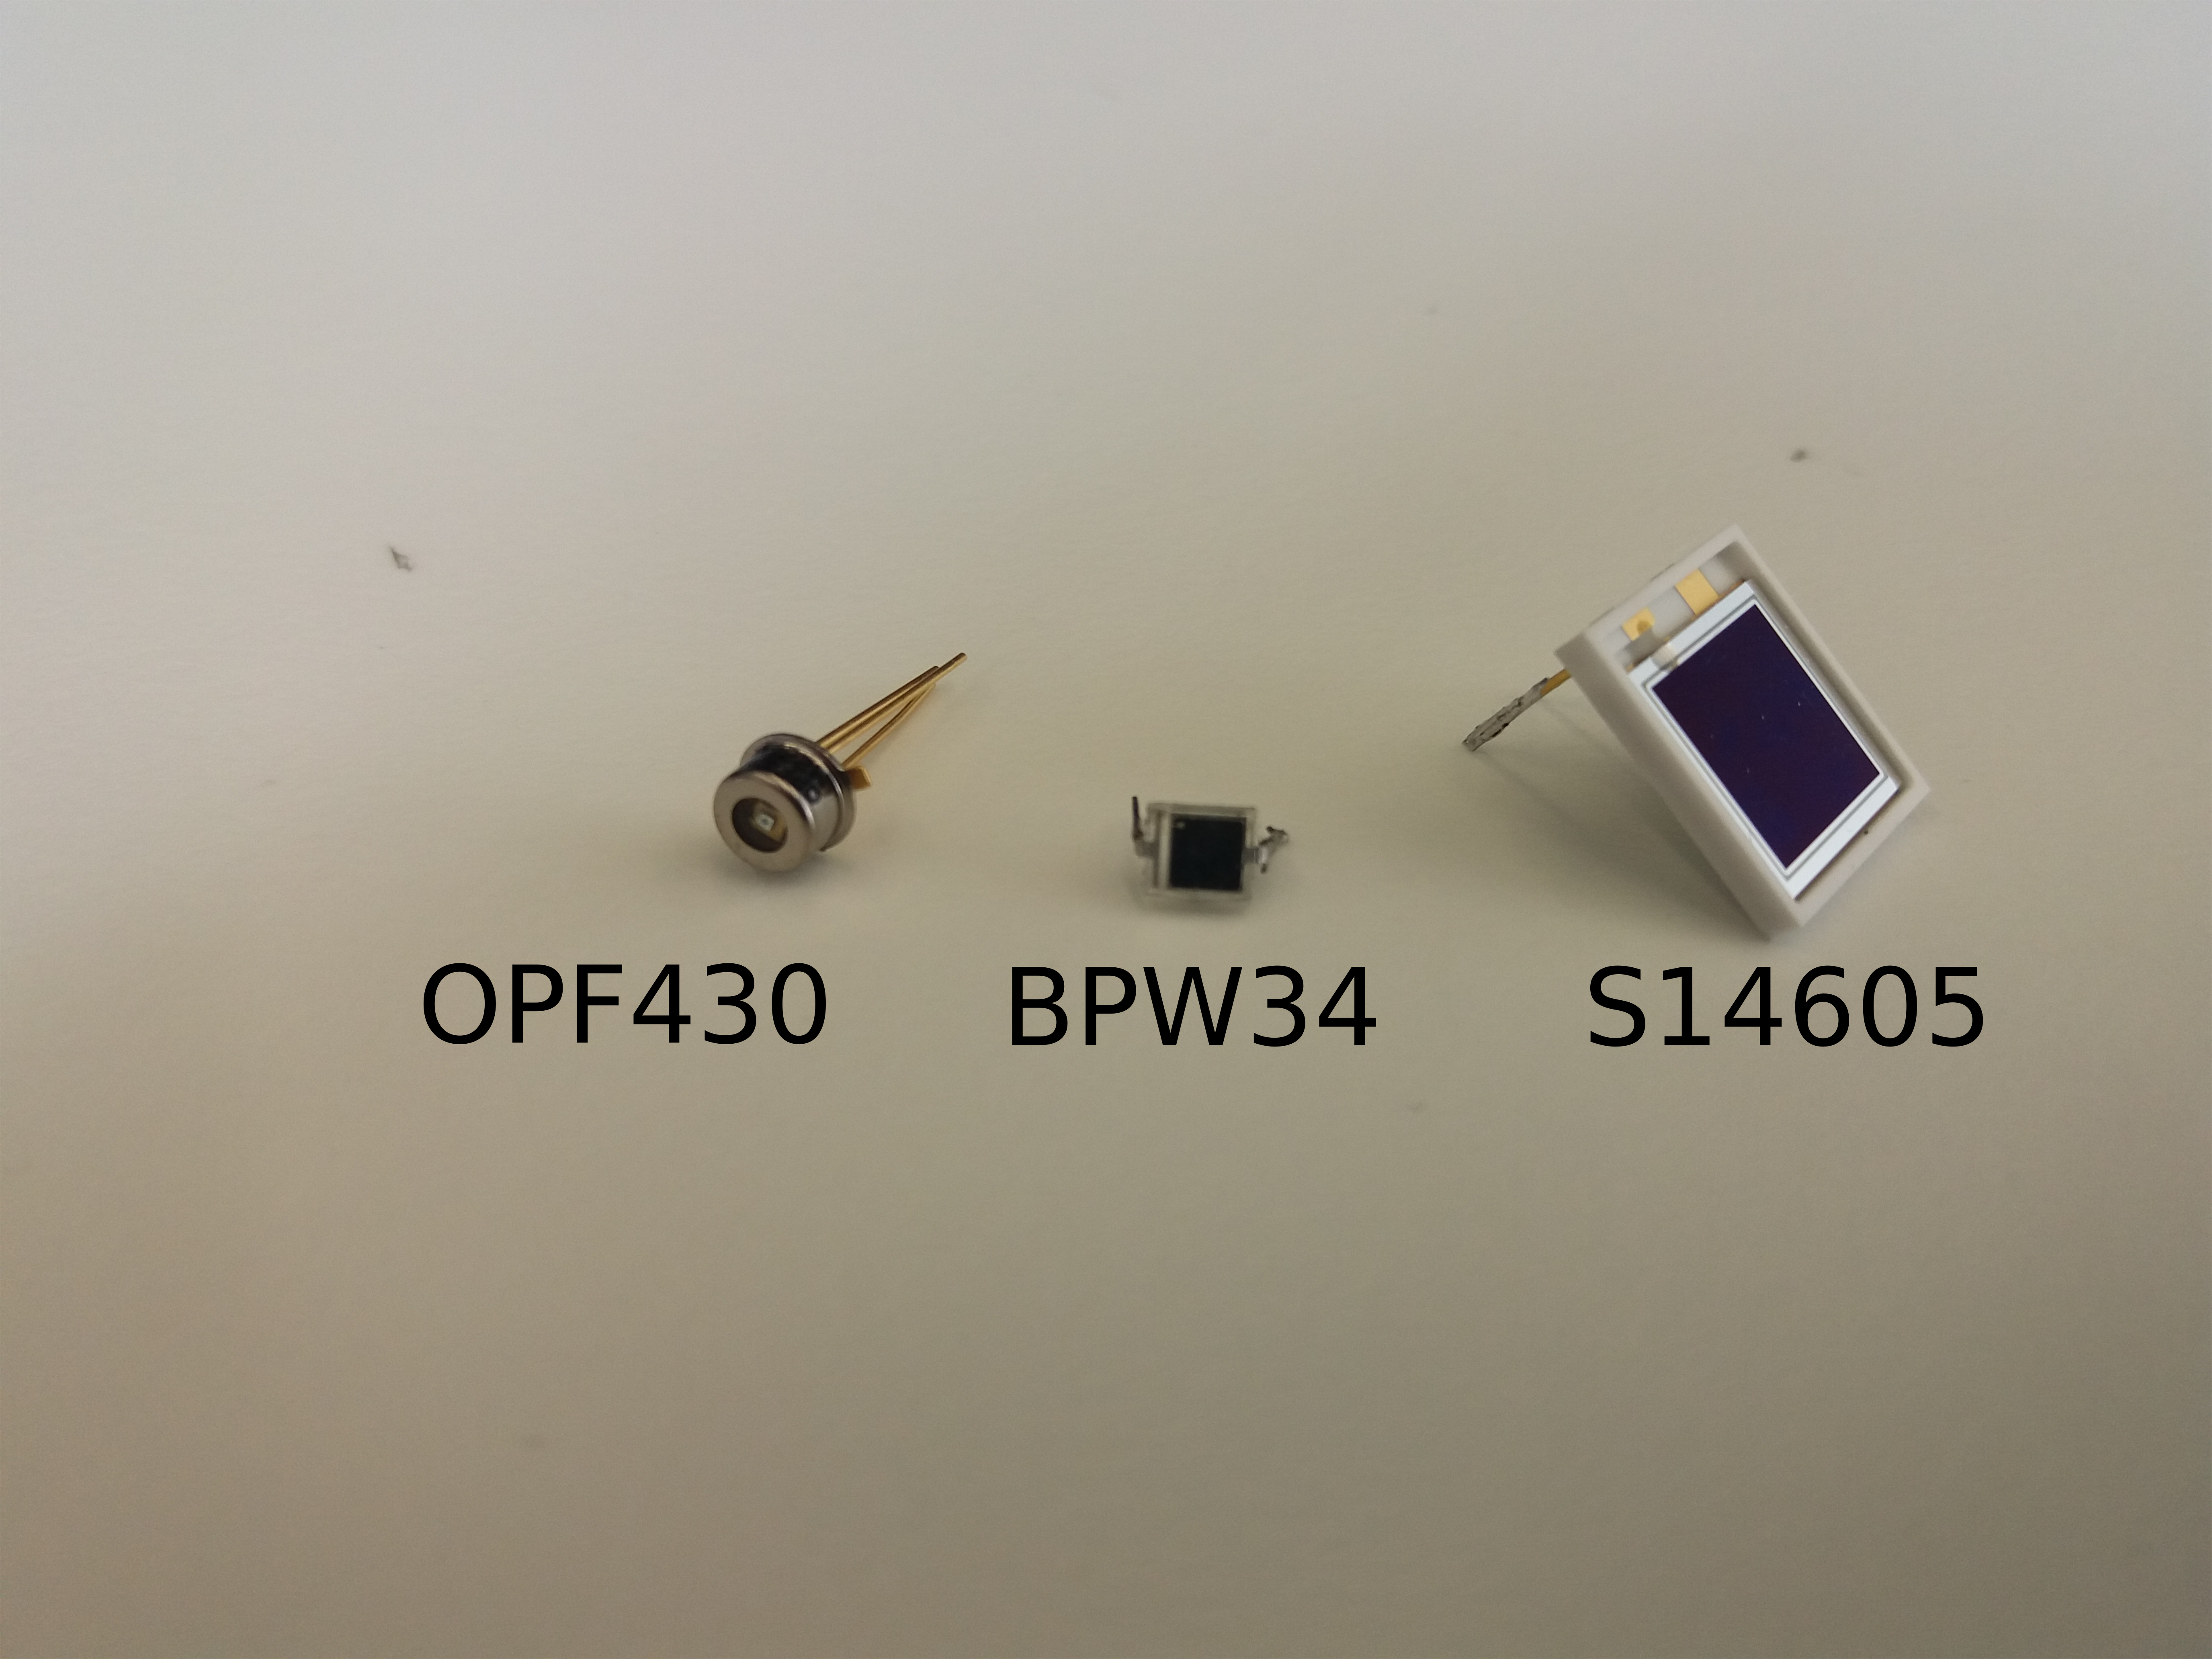
\includegraphics[scale=0.1, angle = 0]{./pictures/PINdiodes.png}
 \caption{PIN diodes - OPF430, BPW34 and S14605.}
 \label{PIN diodes}

\end{figure}

\subsection{Hamamatsu S14605}
The professional S14605 is designed for use as a direct radiation detector. It has a very large light sensitive area and low capacitance.
%The professional S14605 is designed to be used as a direct radiation detector. It offers a very large photosensitive area and a low capacitance.

Parameters \cite{datS14605}:
\begin{itemize}
\item Maximum reverse voltage $U_\textrm{R}$: 150 V
\item Photosensitive area: 81 mm$^2$
\item Capacitance: 25 pF at $U_\textrm{R} = 100$ V
\item Dark current: 8 nA at $U_\textrm{R} = 100$ V
\item Depletion layer: 0.5 mm
\item Cost: 5000 CZK
\end{itemize}

%\begin{figure}[H]
% \centering
% \includegraphics[scale=0.35, angle = 0]{./pictures/NoPicture.jpg}
% \caption{Hamamatsu S14605.}
% \label{S14605}
% 
%\end{figure}



\subsection{BPW34}
BPW34 is a very inexpensive radiation detector. There was a manual \cite{betaBPW} on how to use BPW34 as a beta particle detector, and since it is a Si PIN diode, it is worth a try and test for our gamma detection purposes.
%BPW34 is a very low cost radiation detector. There was manual \cite{betaBPW} how to use BPW34 as a beta particle detector, and since it is a Si PIN diode, it worths a try and test it for our gamma detection purposes.



Parameters \cite{datBPW34}:
\begin{itemize}
\item Maximum reverse voltage $U_\textrm{R}$: 32 V
\item Photosensitive area: 7.5 mm$^2$
\item Capacitance: 25 pF at $U_\textrm{R} = 3$ V
\item Dark current: 2 nA at $U_\textrm{R} = 10$ V
\item Depletion layer: not specified
\item Cost: 11 CZK
\end{itemize}

%\begin{figure}[H]
% \centering
% \includegraphics[scale=0.35, angle = 0]{./pictures/NoPicture.jpg}
% \caption{BPW34.}
% \label{BPW34}
% 
%\end{figure}
\subsection{OPF430}
OPF430 was originally intended as a low cost detector for fibre optic applications. However, there was a publication \cite{RAMIREZJIMENEZ2003577} which described the possibility of using similar diode OPF420 in low energy gamma spectroscopy chains as a low cost detector.
%OPF430 is originally ment to be a low-cost detector for fiber optic applications. However, there was publication \cite{RAMIREZJIMENEZ2003577}, which described the possibility of using similar diode OPF420 in low-energy gamma spectroscopy chains as a low-cost detector.

Parameters \cite{datOPF430}:
\begin{itemize}
\item Maximum reverse voltage $U_\textrm{R}$: 100 V
\item Photosensitive area: not specified, smaller than BPW34
\item Capacitance: 1.5  pF at $U_\textrm{R} = 5$ V
\item Dark current: 0.1 nA at $U_\textrm{R} = 5$ V
\item Depletion layer: not specified
\item Cost: 340 CZK
\end{itemize}

%\begin{figure}[H]
% \centering
% \includegraphics[scale=0.35, angle = 0]{./pictures/NoPicture.jpg}
% \caption{OPF430.}
% \label{OPF430}
% 
%\end{figure}
% %%%%%%%%%%%%%%%%%%%%%%%% End of file %%%%%%%%%%%%%%%%%%%%%%%%


% -----------------------------------------------
% Vlastní text práce (kapitoly práce)
% -----------------------------------------------

% -----------------------------------------------
\chapter{Mössbauer effect and spectroscopy}
% -----------------------------------------------
The Mössbauer effect is an interaction that can occur on atomic nuclei under certain circumstances. It is a recoilless resonance emission/absorption of gamma photons by nuclei of the source/absorber with discrete nuclear energy levels. This effect has a special application in material science - Mössbauer spectroscopy (MS), which is a nuclear experimental technique and a special type of gamma spectroscopy that uses the appropriate nuclei in the sample as probes of local electric and magnetic fields. 

\par
This technique is capable of providing much unique information in material science, geology, chemistry and biology - study of phase and chemical composition of solid materials, study of local magnetic fields and spin states and in-situ measurements of phase transitions \cite{moss}. The main disadvantage of this technique is that there is no suitable radiation source for many isotopes. The most important is iron and its isotope $^{57}$Fe with the radioactive source $^{57}$Co (which decays to an excited state of $^{57}$Fe with a half-life of 271.81 days \cite{co57}), which allows Mössbauer spectroscopy to be used in many areas studying iron compounds.
%Mössbauer effect is an interaction, which can, under certain circumstances, occur on atomic nuclei. It is recoilless resonance emission/absorption of gamma photons by nuclei of source/absorber with discrete nuclear energy levels. This effect has a special application in the field of material research - the Mössbauer spectroscopy (MS), which is a nuclear experimental technique and a special type of gamma spectroscopy, which uses the appropriate nuclei in studied sample as probes of local electric and magnetic fields. 
%
%\par
%This technique is capable of providing many unique information in material research, geology, chemistry and biology - study of phase and chemical composition of solid materials, study of local magnetic fields and spin states and in-situ measurements of phase transitions \cite{moss}. The main disadvantage of this technique is the fact that there is not an appropriate radiation source for many isotopes. The major significance has iron and its isotope $^{57}$Fe with radioactive source $^{57}$Co (which decays into an excited state of $^{57}$Fe with half-life 271.81 days \cite{co57}), which allows the Mössbauer spectroscopy to be employed in many fields investigating iron compounds.

% -----------------------------------------------
\section{Physical concept}

\subsection{Resonace emission and absorption}
In the previous chapters it was mentioned that atomic nuclei are quantum systems with discrete energy levels (analogous to the energy levels of the electron shell), so upon de-excitation or excitation they emit/absorb gamma photons with energy $E_0$ equal to the difference between the levels. The emitted/absorbed energy spectra follow the shape of the Lorentzian curve. 
\par
However, these emitted/absorbed energy spectra are altered due to the momentum conservation law. Part of the gamma photon energy is transferred to the kinetic energy of the nucleus, the crystal as a whole body, or transformed into lattice vibrations (phonons). 
In the case of a free, stationary nucleus, the momentum and energy transfers are so large that the emission and absorption spectra are shifted in different directions by large energetic values, making resonance absorption impossible to observe. However, the case of the nucleus bounded in the crystal lattice is different - the crystal as a whole body will absorb the momentum. If we consider that the whole crystal has a much larger mass than the nucleus, the energy transfer into the kinetic energy of the crystal will be negligible - the gamma photon energy remains unchanged and this results in recoilless emission/absorption. In this case the emission and absorption energy spectra overlap and this makes resonance absorption (Mössbauer effect) observable \cite{moss}.
%In previous chapters was mentioned, that the atomic nuclei are quantum systems with discrete energy levels (analogous to the energy levels of electron shell), thus upon deexcitation or excitation they emit/absorb gamma photon with energy $E_0$ equal to the difference between the levels. The emitted/absorbed energy spectra follow the shape of Lorentzian curve. 
%\par
%However, these emitted/absorbed energy spectra are altered due to the  momentum conservation law. Part of the gamma photon energy is transferred to the  kinetic energy of nucleus, crystal as whole body or is transformed into lattice vibrations (phonons). 
%In the case of free, stationary nucleus, momentum and energy transfers are so high, that the emission and absorption spectra are shifted to different directions by large energetic values, which makes the resonance absorption impossible to observe. However, the nucleus bounded into the crystal lattice is a different case - the crystal as whole body will absorb the momentum. If we consider, that the entire crystal has much larger mass than the nucleus, the energy transfer into kinetic energy of the crystal will be negligible - the gamma photon energy remains unaltered and that results into recoilless emission/absorption. In this case the  emission and absorption energy spectra have overlap and that makes the resonance absorption (Mössbauer effect) observable \cite{moss}.

\subsection{Interaction of nuclei with local fields}
The nucleus, bounded within the lattice and surrounded by electrons arranged according to the chemical bonds, has perturbed energy levels. These perturbed energy levels are a consequence of the interactions of the nucleus with local electric and magnetic fields, resulting in each phase or chemical composition having its own nuclear emission/absorption spectrum - the Mössbauer spectrum. Quantum physics has very well known calculation techniques to describe these variations in energy spectra - perturbation theory.

\par
The main properties of a nucleus that cause the interactions with local electric and magnetic fields are: the atomic number $Z$, the quadrupole moment $Q$ and its spin $I$ along with its projections. For spectroscopy there are three main hyperfine interactions \cite{moss}:

\begin{itemize}
\item Electric monopole interaction - the interaction between the protons of the nucleus and the s-electrons (which have a non-zero probability of being in the nucleus). It results in an isomeric shift of the energy levels $\delta = E_M - E_0$. The $\delta$ must be defined with respect to a fixed energy level, for example the level of the radioactive source that is used. This type of MS spectrum has a shape consisting of only one Lorentzian (singlet shape).
\item Electric quadrupole interaction - the inhomogeneous electric field inside the nucleus interacts with the quadrupole momentum $Q$ of the nuclei. It results in energy variations with respect to the square of the magnetic quantum number $E_Q \sim m^{2}$ - the states allowing different values of $|m|$ are split into sub-states. For $m = \pm 1/2$ there are two Lorentzians in the MS spectra - dublet.
\item Magnetic dipole interaction - the spin $I$ is tied to the magnetic momentum by the relation $\mu = \gamma I$, where $\gamma$ is a gyromagnetic ratio. This magnetic momentum interacts with magnetic fields in the nucleus and leads to the nuclear Zeeman effect - the splitting of states with respect to possible values of the magnetic quantum number $m$. The magnetic dipole interaction plays an important role in studying the magnetic properties of materials.
\end{itemize}
Each of these effects can occur separately or simultaneously with the others.
%The nucleus bounded inside the lattice surrounded by electrons arranged according to the chemical bonds has perturbed energy levels. These perturbed energy levels are consequences of the interactions of nucleus with local electric and magnetic fields, resulting in each phase or chemical composition has its own nuclear emission/absorption spectrum - the Mössbauer spectrum. The quantum physics has very-well known computation techniques to describe these variations in energy spectra - the perturbation theory.
%
%\par
%The main properties of nucleus which induces the interactions with local electric and magnetic fields are: atomic number $Z$, quadrupole momentum $Q$ and its spin $I$ along with its projections. For spectroscopy there are three main hyperfine interactions \cite{moss}:
%
%\begin{itemize}
%\item Electric monopole interaction - the interaction between the protons of nucleus and the s-electrons (which have non-zero probability of being found inside nucleus). It results into isomer shift of energy levels $\delta = E_M - E_0$. The $\delta$ has to be defined with respect to some fixed energy level, for example to the level of the used radioactive source. This type of MS spectra has shape consisting of only one Lorentzian (singlet shape).
%\item Electric quadrupole interaction - the inhomogeneous electric field inside nucleus interacts with the quadrupole momentum $Q$ of the nuclei. It results into energy variations with respect to the square of magnetic quantum number $E_Q \sim m^{2}$- the states which allows different values of $|m|$ are splitted into sub-states. For $m = \pm 1/2$ there are two Lorentzians in MS spectra - dublet. 
%\item Magnetic dipole interaction - the spin $I$ is tied up with magnetic momentum via relation $\mu = \gamma I$, where $\gamma$ is a gyromagnetic ratio. This magnetic momentum interacts with magnetic fields inside nucleus and results into nuclear Zeeman effect - the splitting of the states with respect to possible values of magnetic quantum number $m$. The magnetic dipole interaction has a significant role when it comes to study the magnetic properties of materials.
%\end{itemize}
%Each of these effects can occur separately or simultaneously with the others.


% -----------------------------------------------



\section{Mössbauer spectroscopy}
To obtain the spectra, we can use one of several measurement setups with given geometries. In laboratories there are dominant the setups employing transmission or backscattering geometry with the sample as the absorber and with Doppler modulation of the gamma photon energy. The emitted photons or other products generated by the excitation are detected by a detector with electronics to accumulate the Mössbauer spectra. The source is attached to the Doppler modulation unit (transducer) and the energy of the gamma photons is modulated by the relative velocity of the source and absorber, typically in the range of about $\pm$ 1 $\mu$eV.
\par
For the transmission geometry, the key concept of the measurement is that if we irradiate the sample placed as an absorber with gamma photons with energy varied by the Doppler modulation, the gamma photons with energy equal to one of the transitions (resonance energies) will be absorbed with a certain probability. The detector is positioned behind the absorber and measures the number of gamma photons at a defined energy step. The minimum counts are measured around the resonance energy. The transmission geometry of Mössbauer spectra can be seen in the figure \ref{msspec}.
%To obtain the spectra, we can use one of the several measurement setups with given geometries. In laboratories there are dominant the setups employing transmission or backscattering geometry with sample as an absorber and with the Doppler modulation of the gamma photons energy. The transmitted photons or other products developed upon deexcitation are detected by appropriate detector with electronics to accumulate the Mössbauer spectra. The source is attached to the Doppler modulation unit (transducer), and by the relative velocity of source and absorber the energy of gamma photons is modulated typically in the range of about $\pm$ 1 $\mu$eV.
%\par
%For transmission geometry the key concept of measurement is that if we irradiate the sample placed as an absorber by gamma photons with energy varied by the Doppler modulation, the gamma photons with energy equal to one of the transitions (resonant energies) are absorbed with certain probability. The detector is situated behind the absorber and measures the number of gamma photons at defined energy step. The minimum counts are measured around the resonant energy. The transmission geometry Mössbauer spectra can be seen in the figure \ref{msspec}.
\par
The concept of a backscattering geometry is similar in many ways, but the main difference is the detection of the secondary particles. The nuclei in the sample are excited by appropriate gamma photons and subsequently decay back to the original state with some effects following - re-emission of the "original" gamma photons in a random direction, emission of electrons from the shell (ejected by deexcitation energy quanta, also called conversion electrons) followed by characteristic x-rays or possibly by auger electrons. The detection of electrons and X-rays instead of gamma photons has many advantages and disadvantages, and for certain applications the use of the backscattering geometry may be more appropriate. For example, the detection of conversion electrons could handle the surface characterisation of the sample due to the lower transmittance of electrons when compared to gamma photons.
%\par
%The concept of backscattering geometry is similar in many ways, but the main difference is the detection of the secondary particles. The nuclei in the sample are excited by appropriate gamma photons and subsequently, they decay back into the original state with some effects following - reemission of the "original" gamma photons in random direction, emission of electrons from the shell (ejected by deexcitation energy quanta, also called conversion electrons) followed by characteristic x-rays or possibly by auger electrons. The detection of electrons and x-rays instead of gamma photons have many advantages and disadvantages and for certain application, the usage of backscattering geometry could be more appropriate. For example, the detection of conversion electrons could handle the surface characterization of the sample due to the lower transmittance of electrons when compared to gamma photons.

\begin{figure}[H]
 \centering
 \includegraphics[scale=0.7, angle = 0]{./pictures/MSSpec.png}
 \caption{Transmission Mössbauer spectrum of $\alpha$-Fe. Taken and modified from \cite{NOVAK2016thesis}.}
 \label{msspec}
 
\end{figure}


\section{$^{57}$Fe spectroscopy}
One of the isotopes on which we are able to observe a Mössbauer effect is $^{57}$Fe (relative abundance only $2.119 \%$ \cite{compounds}). The source is $^{57}$Co, which decays into the second excited state of $^{57}$Fe by electron capture. The resulting $^{57}$Fe nuclei can deexcite themselves in two ways ( figure \ref{Fe57scheme}) - by direct deexcitation to the ground state by emission of 136.5 keV photon or by deexcitation to the first excited state by emission of 122.1 keV photon. The first excited state is essential as it is used to study the hyperfine interactions. After the lifetime of the first excited state, the 14.4 keV photon (or other possible conversion products) is emitted as it falls to the ground state. The $^{57}$Fe spectroscopy in transmission geometry is based on the detection of the 14.4 keV gamma photons. This thesis is mainly devoted to the application of semiconductor detectors for the detection of these 14.4 keV gamma photons. The $^{57}$Fe spectroscopy can also be performed in the backscattering geometry by detecting the conversion electrons or conversion X-rays with energies around 6.4 keV.
%One of the isotopes, on which we are capable to observe a Mössbauer effect is $^{57}$Fe (relative abundance only $2.119 \%$ \cite{compounds}). As a source is used $^{57}$Co, which decays into second excited state of $^{57}$Fe by electron capture. The originated $^{57}$Fe nuclei can deexcite itself by two ways (figure \ref{Fe57scheme}) - by direct deexcitation onto the ground state by emission of 136.5 keV photon or by deexcitation onto the first excited state by emission of 122.1 keV photon. The first excited state is essential since it is used to study the hyperfine interactions. After the lifetime of the first excited state the 14.4 keV photon is emitted (or other possible conversion products) when falling into the ground state. The $^{57}$Fe spectroscopy in transmission geometry is based on detection of the 14.4 keV gamma photons. This thesis is mainly devoted to the application of semiconductor detectors for the detection of these 14.4 keV gamma photons. The $^{57}$Fe spectroscopy can also be performed in backscattering geometry by the detection of the conversion electrons or conversion x-rays with energies around 6.4 keV.

\begin{figure}[H]
 \centering
 \includegraphics[scale=0.75, angle = 0]{./pictures/Fe57}
 \caption{Decay scheme of $^{57}$Co, taken from \cite{NOVAK2016thesis}.}
 \label{Fe57scheme}
 
\end{figure}

The MS spectrometer setup consists of several parts:
\begin{itemize}

\item Source of 14.4 keV gamma - $^{57}$Co radioactive nuclei built into a crystal lattice (usually in a rhodium matrix). The source is mounted on the transducer.
\item Transducer for Doppler modulation (figure \ref{transducer}). It usually consists of two coils surrounded by permanent magnets - one to drive the Doppler energy modulation and the other to measure the velocity \cite{mossInstr}. The system is driven by PID (proportional integral derivative) or MPC (model predictive control) controllers for precise velocity and energy control. The speed can be either constant or with constant acceleration.

\item Detector of transmitted/backscattered gamma radiation, conversion electrons or X-rays together with readout and evaluation electronics including amplifiers, single or multi-channel analysers, etc. It should also be noted that the conventional detectors mentioned above do not have sufficient energy resolution to distinguish the energy of perturbed states. For this reason, the count rates are synchronised with the Doppler energy modulation (actual modulated energy of the source), which is used to address the channels for spectrum accumulation. 


\end{itemize}
%The MS spectrometer setup consist of several parts:
%\begin{itemize}
%
%\item Source of 14.4 keV gamma - $^{57}$Co radioctive nuclei built-in crystal lattice (mostly in a rhodium matrice). The source is attached to the transducer.
%\item Transducer for doppler modulation (figure \ref{transducer}). It mostly consists of two coils surrounded by permanent magnets - one for driving the Doppler energy modulation and second for the velocity measurement \cite{mossInstr}. The system is driven by PID (proportional integral derivative) or MPC (model predictive control) controller for precise velocity and energy control. The velocity can be either constant or with constant acceleration.
%
%\item Detector of transmitted/backscattered gamma radiation, conversion electrons or X-ray along with readout and evaluation electronics including amplifiers, singlechannel or multichannel analysers etc. It is also necessary to consider, that the already mentioned conventional detectors have not sufficient energy resolution to distinguish the energy of perturbed states. Because of that, the count rates are synchronised with the Doppler energy modulation (actual modulated energy of the source), which is used to address the channels for spectra accumulation. 
%
%
%\end{itemize}

\begin{figure}[H]
 \centering
 \includegraphics[scale=0.4, angle = 0]{./pictures/transducer}
 \caption{Transducer, taken from \cite{STEJSKAL2019thesis}.}
 \label{transducer}
 
\end{figure}


The diagram of the MS setup can be seen in the figure \ref{diagram}.

\begin{figure}[H]
 \centering
 \includegraphics[scale=0.8, angle = 0]{./pictures/MSsetup.png}
 \caption{Diagram of the MS setup, taken and modified from \cite{NOVAK2016thesis}.}
 \label{diagram}
 
\end{figure}


\section{MS spectra effect and SNR}
The shape of the MS spectra can be modelled by Lorentzian curves. The singlet spectra in transmission geometry can be modelled by a single Lorentzian curve of the following form:

\begin{equation}
\begin{aligned}
L(v) = -I_{\textrm{MS}}\frac{(\frac{\Gamma}{2})^2}{(v - v_0)^2 + (\frac{\Gamma}{2})^2} + B
\end{aligned},
\label{lor}
\end{equation}
where $I_{\textrm{MS}}$ is the amplitude, the $\Gamma$ is the FWHM, and the $B$ is a background level. The Lorentzian in this form has the associated area $A$ equal to:

\begin{equation}
\begin{aligned}
A = \pi I_{\textrm{MS}} \Gamma
\end{aligned}
\label{area}
\end{equation}

There are two properties of MS spectra that characterise their quality: SNR and the effect $E_{\textrm{MS}}$. They can be calculated from the spectrum parameters using the following equations:

\begin{equation}
\begin{aligned}
\textrm{SNR}_{\textrm{MS}} = \frac{I_{\textrm{MS}}}{\sqrt{B}}
\end{aligned}
\label{SNR}
\end{equation}

\begin{equation}
\begin{aligned}
E_{\textrm{MS}} = \frac{I_{\textrm{MS}}}{B}
\end{aligned}
\label{effect}
\end{equation}



% %%%%%%%%%%%%%%%%%%%%%%%% End of file %%%%%%%%%%%%%%%%%%%%%%%%


% -----------------------------------------------
% Vlastní text práce (kapitoly práce)
% -----------------------------------------------

% -----------------------------------------------
\chapter{Electronics for signal readout and analysis}
% -----------------------------------------------
The signals coming out of the detector have to be properly preamplified, amplified and shaped. This  task requires special analog circuits with properly designed layout. 
The measurement chain for gamma spectroscopy is usually realized in following order - gamma detector, preamplifier, amplifier, multichannel analyser (MCA), microprocessor/computer (figure \ref{chain}). When designing this spectrometric chain, we select components in order to achieve sufficient parameters for certain application - in our case the energy resolution. For our spectrometric chain we chose instruments, modules and parts from two companies - ORTEC and CREMAT.

\begin{figure}[H]
 \centering
 \includegraphics[scale=0.35, angle = 0]{./pictures/chain.png}
 \caption{Spectrometric chain.}
 \label{chain}
 
\end{figure}


\par
The task of realizing the spectrometric chain can be fulfilled in two ways. The first and more straightforward way is to build it from stand-alone robust instruments and modules. The second possibility is to design printed circuit board (PCB) with required functionalities from electronic components. In this thesis, we apply both methods for the development. 
\par
Building the chain from the stand-alone instruments can be more practical approach for testing of the detectors themselves since we are not forced to solve problems arising from the design of the board of the electronic circuit. However, these modules are usually very expensive, measurement setups build this way are unnecessarily large and have worse noise parameters than electronic circuits specially tailored for the given application.
\par
Designing the PCB requires many electronic engineering skills and time for development. The analog PCBs are very hard to design. The pros are that the final product can be very compact and cheap to manufacture.



\section{PIN detector connection and bias voltage}
\subsection{Voltage source}
The PN and PIN detectors require voltage bias to reduce the capacitance.
These voltage sources don't have to be stiff since the current consumption of the detector is very low.
\par
Gas and scintillation detectors usually require high voltage sources (hundreds or thousands of volts). These high voltages are usually delivered by switching power supplies.
However, these supplies are usually very noisy and since the semiconductors can be operated at much lower voltages, there is no need for them. The better alternative is charge pump build of capacitors and diodes, which requires lower frequencies to operate.
\subsection{Shielding and grounding}

In case of sensitive analog signal circuits, the electromagnetic shielding is a very important part. Sensitive circuits have to be surrounded by a metallic material from all sides, which is also correctly connected to GND (principle of the Faraday cage), otherwise the proper functionality can not be guaranteed. The electromagnetic disturbance usually induces currents in the shielding material, and thus the special care has to be taken to prevent these currents from flowing through the signal routes. The figure \ref{shielding} shows the difference between correct and wrong connection of shielding.

\begin{figure}[H]
 \centering
 \includegraphics[scale=0.35, angle = 0]{./pictures/shielding.png}
 \caption{Schematic of wrong and correct connection of shielding \cite{appCSPnote}.}
 \label{shielding}
 
\end{figure}



\subsection{Cooling}
To reduce thermal noise and achieve better SNR it is necessary to cool the detector. The cooling can be achieved by various ways. In most setups, the appropriate solution can be provided by a Peltier cooler. These setups with Peltier are the easy to implement, however, their cooling efficiency is highly dependent on the ability to sink the heat from the hot side.

\section{Spectrometric chain components}





\subsection{Pre-amplification}
The signal coming out of the PIN detector is a charge (current pulse), so it is necessary to convert it into voltage pulse. For performing the charge-voltage conversion, there is circuit called charge amplifier (also referred as a preamplifier). The principal functional scheme is described by one opamp with a capacitor in feedback (see figure \ref{trans}). The functionality is similar to $I/U$ transimpedance amplifier, but the charge amplifier works mainly as an integrator. In ideal case (opamp amplification $A >> 0$), the measured voltage per unit charge is approximately equal to:

\begin{equation}
\frac{dU}{dQ} = \frac{1}{C_{f}}.
\end{equation}
\par
In real circuit there is also a resistor parallel to the feedback capacitor. The feedback resistor slowly discharges the capacitor after a accumulation of charge, restoring the transimpedance amplifier to be ready to capture another pulse.

\begin{figure}[H]
 \centering
 \includegraphics[scale=0.4, angle = 0]{./pictures/champlifier.png}
 \caption{Charge ampifier. $Qs$ is total charge of pulse and $to$ is the interval of charge generation inside the detector. Taken from \cite{charge}.}
 \label{trans}
 
\end{figure}





\begin{figure}[H]
 \centering
 \includegraphics[scale=0.4, angle = 0]{./pictures/NoiseEquiv.png}
 \caption{Noise equivalent circuit for charge amplifier. Taken from \cite{charge}.}
 \label{transNoise}
 
\end{figure}


The functionality of charge amplifier is also negatively affected by an electronic noise, which depends on the values of the feedback resistance and capacitance and also on the internal parameters of the connected semiconductor detector and field-effect transistor (FET) inside the amplifier. The noise model of the preamplifier circuit can be seen in the figure \ref{transNoise}. This electronic noise can be divided into three contributions, each described by euqations for noise voltages and currents \cite{charge}:

% on including the detector's capacitance $C_{\textrm{det}}$. Thermal noise dependency on $C_{\textrm{det}}$ of the first-stage FET transistor can be approximated by equation \cite{charge}:
\begin{itemize}
\item Thermal noise of first-stage FET:
\begin{equation}
en_1 = \sqrt{\frac{8}{3}\frac{kT}{g_{\textrm{m}}}},
\end{equation}
where $k$ is the Boltzmann constant, $T$ is the absolute temperature and $g_{\textrm{m}}$ is the transconductance of FET.
\item Shot noise caused by FET's gate current and detector's dark current:
\begin{equation}
in = \sqrt{2e(I_{\textrm{G}} + I_{\textrm{D}})},
\end{equation}
where $e$ is the elementary charge, $I_{\textrm{G}}$ is the gate leakage current of first-stage FET and $I_{\textrm{D}}$ is the dark current of detector.
\item Thermal noise caused by feedback resistance: 
\begin{equation}
en_2 = \sqrt{4KTR_{\textrm{f}}},
\end{equation}
where $R_{\textrm{f}}$ is the feedback resistance.
\end{itemize}
The square of total noise $ent^2(j \omega)$ is given by equation:
\begin{equation}
\begin{aligned}
ent^2(j \omega) = en_1^2 \cdot (1+\frac{C_{\textrm{in}}}{C_{\textrm{f}}})^2 + \{in^2 + (\frac{en_2}{R_{\textrm{f}}})^2 \}\frac{1}{(j \omega C_{\textrm{f}})^2},
\end{aligned}
\label{finalNoise}
\end{equation}
where the $C_{\textrm{f}}$ is the feedback capacitance and $C_{\textrm{in}}$ is the total input capacitance, resulting capacitance on the input of amplifier (there - parallel combination of detector's capacitance $C_{\textrm{j}}$ and amplifier's input capacitance $C_{\textrm{s}}$).   
\par
The first term in equation \ref{finalNoise} depends on the ration between the input capacitance $C_{\textrm{in}}$ and the feedback capacitance $C_{\textrm{f}}$ and thus the preamplifier's feedback capacitance has to be optimized in order to reduce the electronic noise.
\par
The charge sensitive preamplifiers modules usually also contain the second stage - common voltage amplifier. The internal scheme of CR-110-R2 charge amplifier made by Cremat Inc., which we use in the case of PCB design can be seen In the Fig. \ref{internal}.
\par
\begin{figure}[H]
 \centering
 \includegraphics[scale=0.35, angle = 0]{./pictures/CRpreamp.png}
 \caption{Internal scheme of CR-110-R2 charge sensitive preamplifier \cite{cr110}.}
 \label{internal}
 
\end{figure}
The output voltage has the shape of exponential decay with amplitude defined by energy deposited into detector, short rise time (in orders of nanoseconds) and a longer decay constant (microseconds).


CR-110-R2 offers the conversion gain $G = 1.4$ V/pC, decay constant $\tau = 140$ $\mu$s CR-110-R2) and noise (FWHM) in silicon equal to 1.7 keV \cite{cr110}. It can be easily calculated, that for 14.4 keV photon, the output pulse has amplitude equal to $U_{A} = 0.8928$ mV. 
Note that the noise caused by the preamplifier is much larger than the intrinsic fano noise (FWHM = 185.4 eV).


\par
The modular version suitable for our application is ORTEC 142A charge preamplifier with $G = 1.016$ V/pC, $\tau = 500$ $\mu$s and noise in silicon equal to 1.6 keV \cite{ORTECpreamp}. Charge preamplifiers are usually very sensitive devices and can be very easily damaged by electrostatics. 

\par

Since the output of preamplifier is in order of millivolts, it has to be strongly amplified. Very fast and low noise amplifier consisting of multiple opamps is an appropriate solution of this problem.



\subsection{Shaping}

To perform the accurate energy discrimination, the pulse shape has to be altered from exponential decay shape by a shaping circuit. The shaping results into filtering the frequency band (reducing the noise) and also into shortening the long decay times of original exponential shapes. The shorter duration of pulses prevents the negative effect in which is one pulse superimposed onto another (pile-up effect).

\par
The Gaussian shape meets the sufficient parameters of SNR and duration \cite{Shapflify}. This type of shaping is usually achieved by several integration stages. The Cremat module CR-200-1us-R2.1 offers gaussian shaping with shaping time 1 $\mu$s \cite{cr200}. Its simplified internal schematic can be seen on fig.\ref{internal2}. 


\begin{figure}[H]
 \centering
 \includegraphics[scale=0.35, angle = 0]{./pictures/CRshaper.png}
 \caption{Internal scheme of CR-200 Gaussian shaping amplifier \cite{cr200}.}
 \label{internal2}
 
\end{figure}

However, shapers are usually very sensitive on the shape of the input pulse. They expect step-like input pulse. The deviation from the expected shapes may result into undefined shapes on output of the shaper. In modules the shapers are usually integrated along with amplifiers.

\subsection{Multichannel analysis (MCA)}
To obtain the full energy spectra information, it is necessary to measure and digitize pulse height of incoming pulses to perform energy discrimination and increment the corresponding channels. The multichannel analyser (MCA) can be employed for these purposes. The EASY-MCA-2K from ORTEC \cite{MCAOrtec}, which we use in experiments, is capable of processing Gaussian shaped pulses with shaping times from 0.25 $\mu$s to 30 $\mu$s and amplitudes ranging from 0 to +10 V.



% %%%%%%%%%%%%%%%%%%%%%%%% End of file %%%%%%%%%%%%%%%%%%%%%%%%

\chapter{Gamma spectrum software analysis}
As was mentioned before in section \ref{char}, the measured gamma spectrum contains many unwanted artifacts like noise, Compton continuum and edges and additional peaks created by various interactions. To properly obtain the count rates on defined energies, the only way is to perform a numerical analysis of measured data. Locations of energy peaks are to be found for example by their characteristic second derivatives. Absolute count rates are then obtained by Gaussian fitting.


\section{Peak searching procedure}
\label{search}
Many commercial programs use peak searching procedures based on algorithm originally developed by M.A. Mariscotti \cite{MARISCOTTI1967309}. This method is based on the numerical second difference assuming that the background can be approximated only by linear functions and thus it vanishes in case of the second derivative. The second fact is that the searched peaks are Gaussians with their specific second derivatives and thus their positions can be found in local minimums (Gaussians have negative second derivatives since their are concave functions). To reduce noise, the second difference is averaged by defined number of steps.
\par
To determine if the found minimum should be considered as peak position (not as a Compton edge etc.), standard deviation and other additional rules based on number of points in specified intervals can be employed. However, algorithm needs input parameters, which are based on raw estimation of FWHM of searched peaks.
\par
For the analysis of measured gamma spectra, this algorithm was implemented in C++ and used to find full energy peaks and other additional peaks as well. The following figures show the example of measured spectra and its second difference plotted along with its standard deviation. The possible candidates onto peak positions can be observed.
\par


\begin{figure}[H]
 \centering
 \includegraphics[scale=0.105, angle = 0]{./pictures/SecondDerivGraph.png}
 \caption{Second difference of example spectra along with its standard deviation showing possible candidates (green lines).}
 \label{secondDerivative}
 
\end{figure}

\begin{figure}[H]
 \centering
 \includegraphics[scale=0.105, angle = 0]{./pictures/DataGraph.png}
 \caption{Example of measured gamma spectra. Green lines mark the energy peaks found by algorithm.}
 \label{Example}
 
\end{figure}


\chapter{Gamma detection testing}
The purpose of this experiment is to determine the conditions necessary for selected photodiodes to be used as detectors for gamma spectroscopy. Note that some of the selected photodiodes are not intended to be used as gamma-ray detectors. The determination of the detection efficiency will be precisely done in the following chapters. 
\par
For the very first test of the photodiodes, we assembled a spectrometric setup consisting of ORTEC modules including a preamplifier ORTEC142A, a shaping amplifier 575A and a high voltage power supply 556 inside the ORTEC minibin (figure \ref{minibin}). The pulses were captured by ORTEC's EASY-MCA-2K connected to a PC running the MAESTRO Multichannel Analyzer Emulation Software \cite{maestro}. As radioactive source we used $^{57}$Co 50 mCi Mössbauer source (date of production: 3.11. 2016) and therefore it was also necessary to cover the part with radiation source with lead shielding blocks.
%The purpose of this experiment is to determine the conditions necessary for selected photodiodes to be used as detectors for gamma spectroscopy. Note that some of the selected photodiodes are not determined to be used as gamma ray detectors. The determination of the detection efficiency is precisely done in the following chapters. 
%\par
%For the very first test of photodiodes we assembled a spectrometric setup from ORTEC modules including preamplifier ORTEC142A, shaping amplifier 575A and high voltage power supply 556 inside the ORTEC minibin (figure \ref{minibin}). The pulses were captured by EASY-MCA-2K from ORTEC connected to PC running the MAESTRO Multichannel Analyzer Emulation Software \cite{maestro}. As a radioactive source we used $^{57}$Co 50 mCi Mössbauer source (date of production: 3.11. 2016) and thus it was also necessary to cover the part with radiation source with lead shielding blocks.


\begin{figure}[H]
 \centering
 \includegraphics[scale=0.09, angle = 270]{./pictures/ORTECbin.jpg}
 \caption{ORTEC minibin with Easy MCA connected to PC.}
 \label{minibin}
 
\end{figure}


\section{Noise reduction}
When performing gamma spectroscopy measurements, the energy spectra are affected by noise. To reduce the noise as much as possible, two approaches have been tested - shielding the detector in various ways and cooling it.
%When performing gamma spectroscopy measurements, the energy spectra are affected by noise. In order to reduce noise as much as possible, two approaches were tested - shielding the detector by various ways and cooling.
\subsection{Electromagnetic noise reduction}
Photodiodes must be adequately shielded from electromagnetic interference and their distance from the preamplifier input should be as short as possible. The use of poorly shielded diodes leads to high levels of electromagnetic noise, which makes a large part of the energy spectrum unobservable.
\par
Based on many tests, it has been proven that the optimal way to shield the photodiode is to place it in an aluminium box (see figure \ref{crate}). This crate must be as small as possible and connected to the ground potential. However, the front of the crate must be open to allow sufficient transmission of gamma photons to the detector. To preserve the shielding properties, this hole has to be covered with a conductive material. We chose a thin aluminium foil, which has sufficient gamma transmission parameters as well as electromagnetic shielding parameters.
%Photodiodes have to be sufficiently electromagnetically shielded and their distance to the preamplifier input should be as short as possible. Using the diodes with poor shielding leads into high levels of electromagnetic noise, which makes major part of energetic spectra unobservable.
%\par
%Based on many test it was proven that  the optimal way to shield the photodiode is to put it into the aluminium crate (see Figure \ref{crate}). This crate has to be as small as possible and has to be connected to the grounding potential. However, the front side of the crate has to be open to allow the sufficient transmission of gamma photons to the detector. To preserve the shielding properties, this drilled hole has to be still covered by a conductive material. Our choice was a thin aluminium foil, which has sufficient gamma transmission parameters as well as electromagnetic shielding parameters.

\begin{figure}[H]
 \centering
 \includegraphics[scale=0.09, angle = 0]{./pictures/ShieldCrate.jpg}
 \caption{Photodiodes inside aluminium shielding crates.}
 \label{crate}
 
\end{figure}


%\begin{figure}[H]
% \centering
% 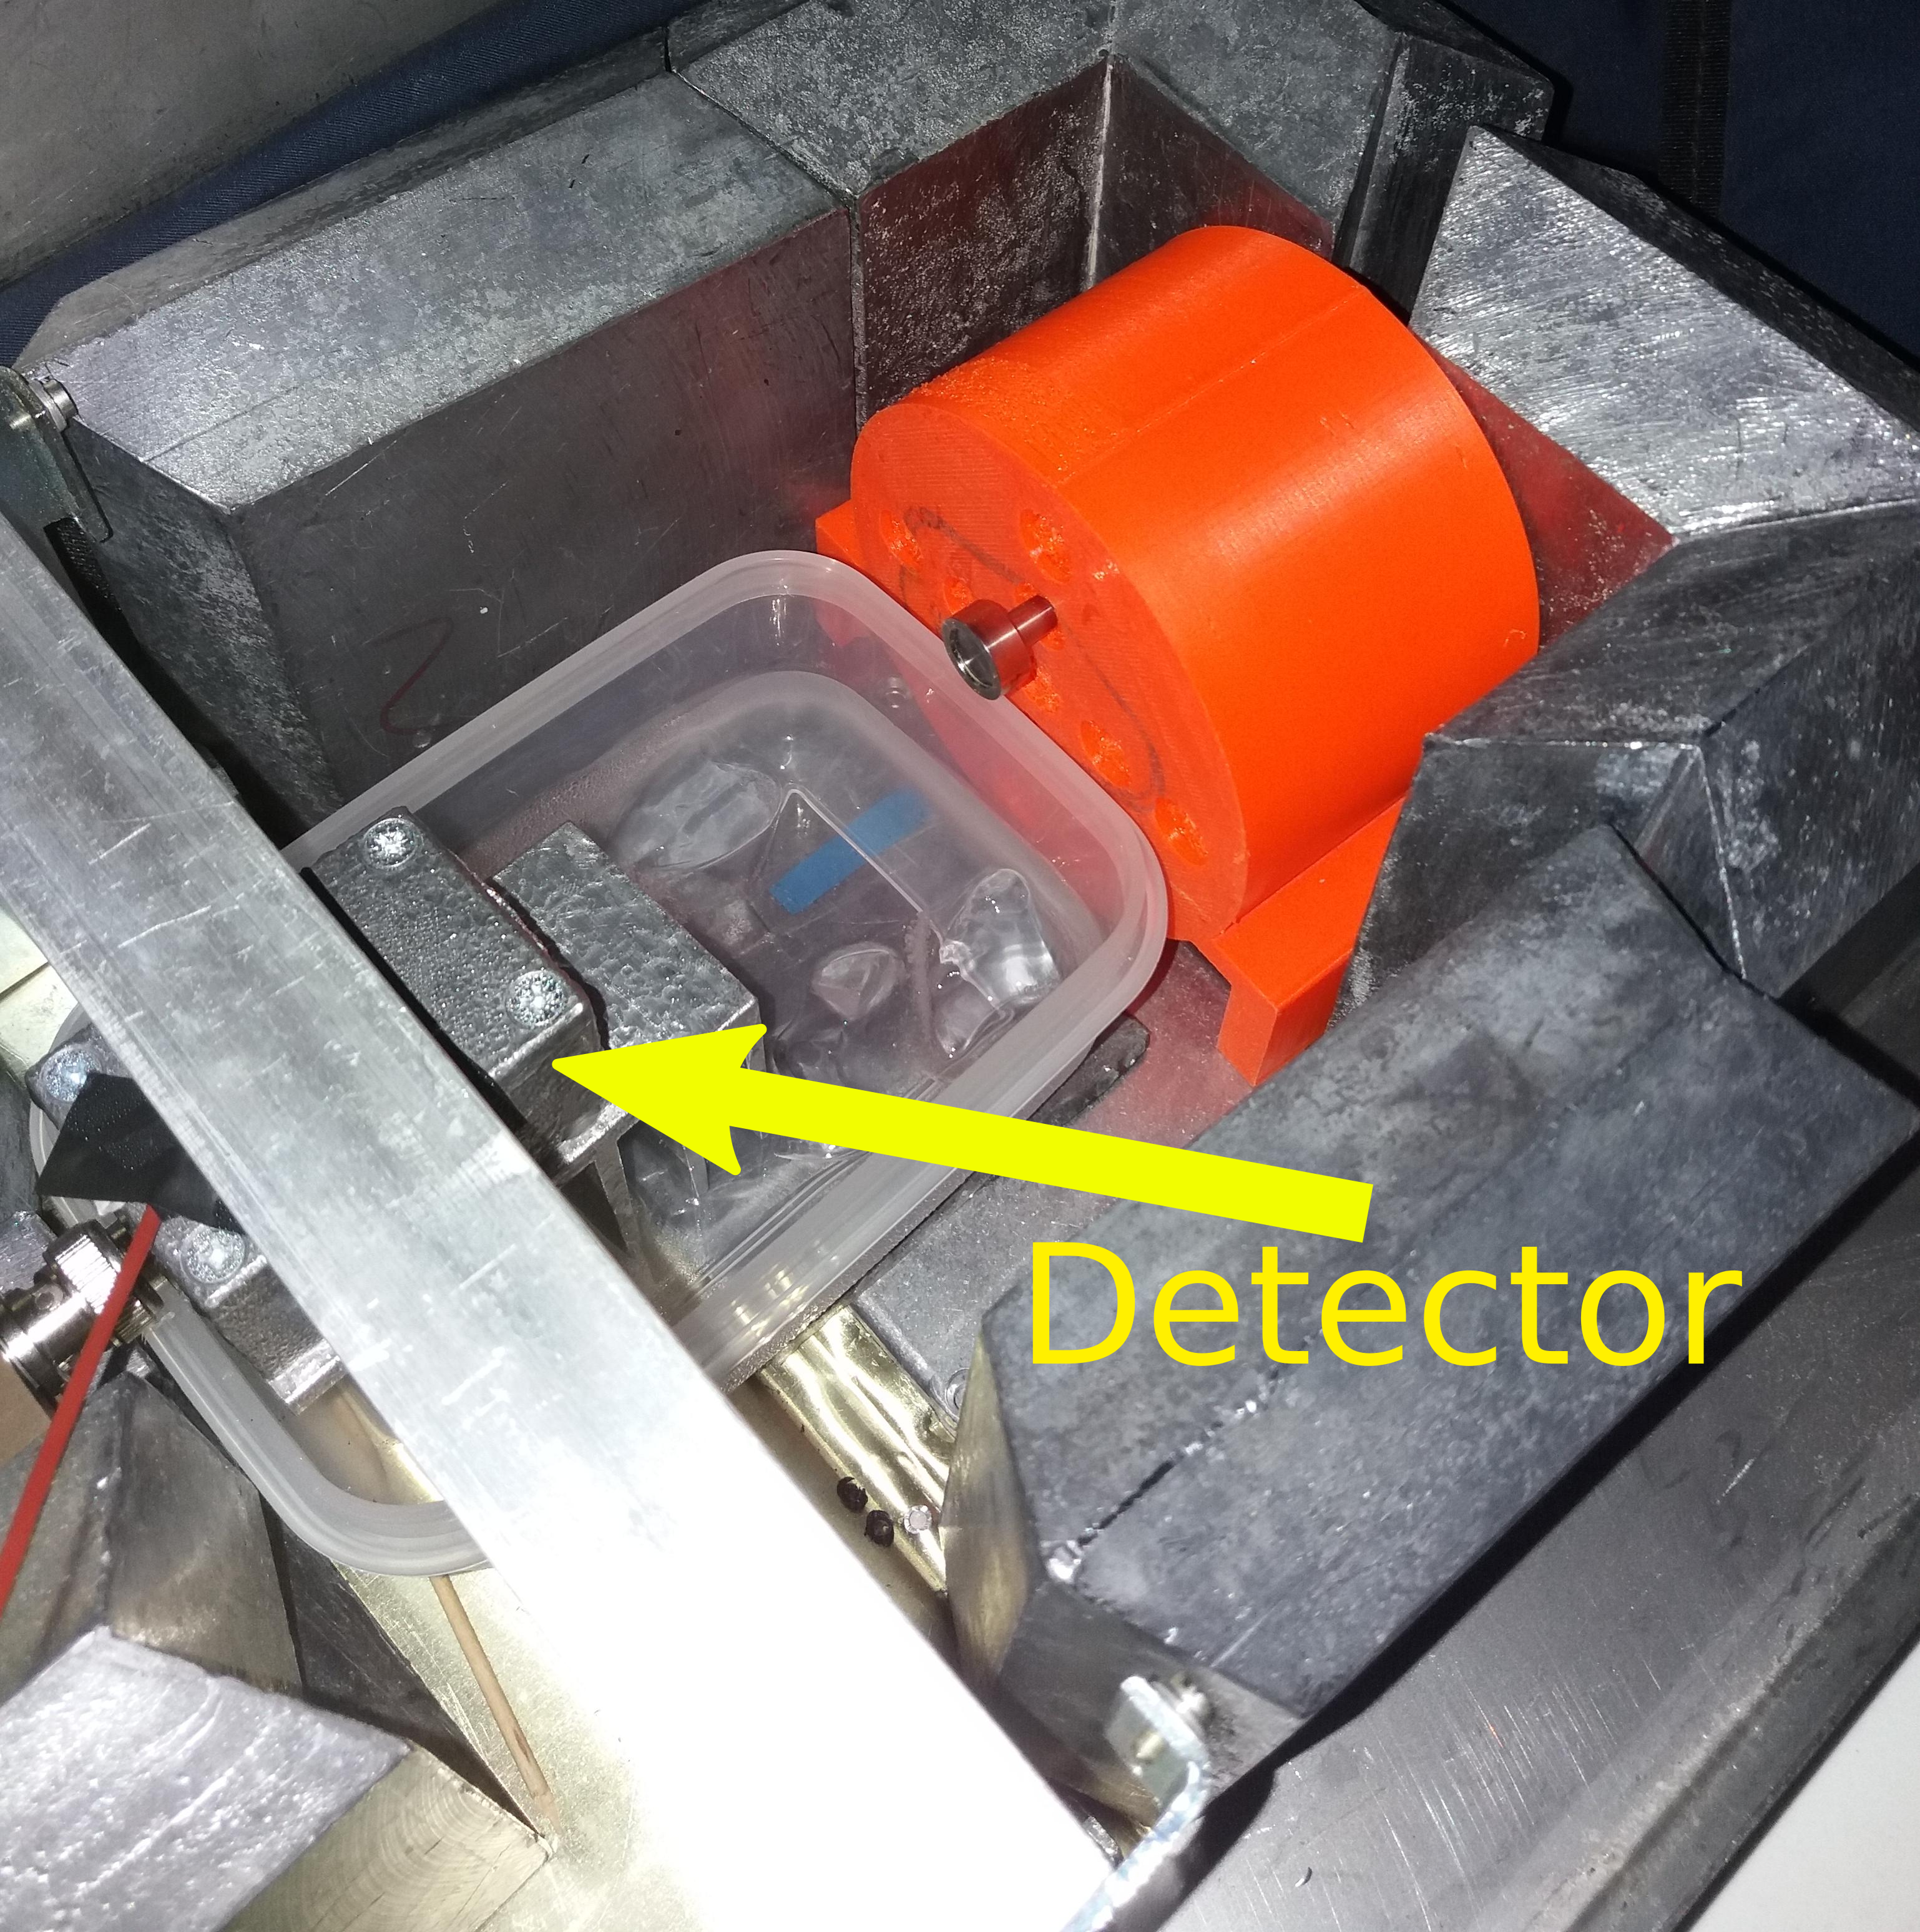
\includegraphics[scale=0.09, angle = 0]{./pictures/chlazeniLedem.jpg}
% \caption{Example of $^{57}$Co spectra from poorly shielded detector setup and from sufficiently shielded detector.}
% \label{notShielded}
% 
%\end{figure}





\subsection{Thermal noise reduction}
To reduce thermal noise, the S14605 photodiode was cooled with ice. It was placed in a shielding box with a heat sink attached to the bottom. This heat sink was submerged in the small tub filled with ice (see figure \ref{cooler}). Thermal conduction was improved by sticking the photodiode to the bottom of the shielding box with thermal paste. The photodiode was cooled in this way to temperatures around 7-8 $^\circ$C.
%To reduce the thermal noise, the S14605 photodiode was cooled by ice. It was placed in shielding box with attached heat sink to the bottom. This heat sink was submerged into the small tub filled with an ice (see Figure \ref{cooler}). The thermal conduction was improved by sticking the photodiode to the floor of the shielding box by a thermal paste. The photodiode was cooled this way to temperatures around 7-8 $^\circ$C.


\begin{figure}[H]
 \centering
 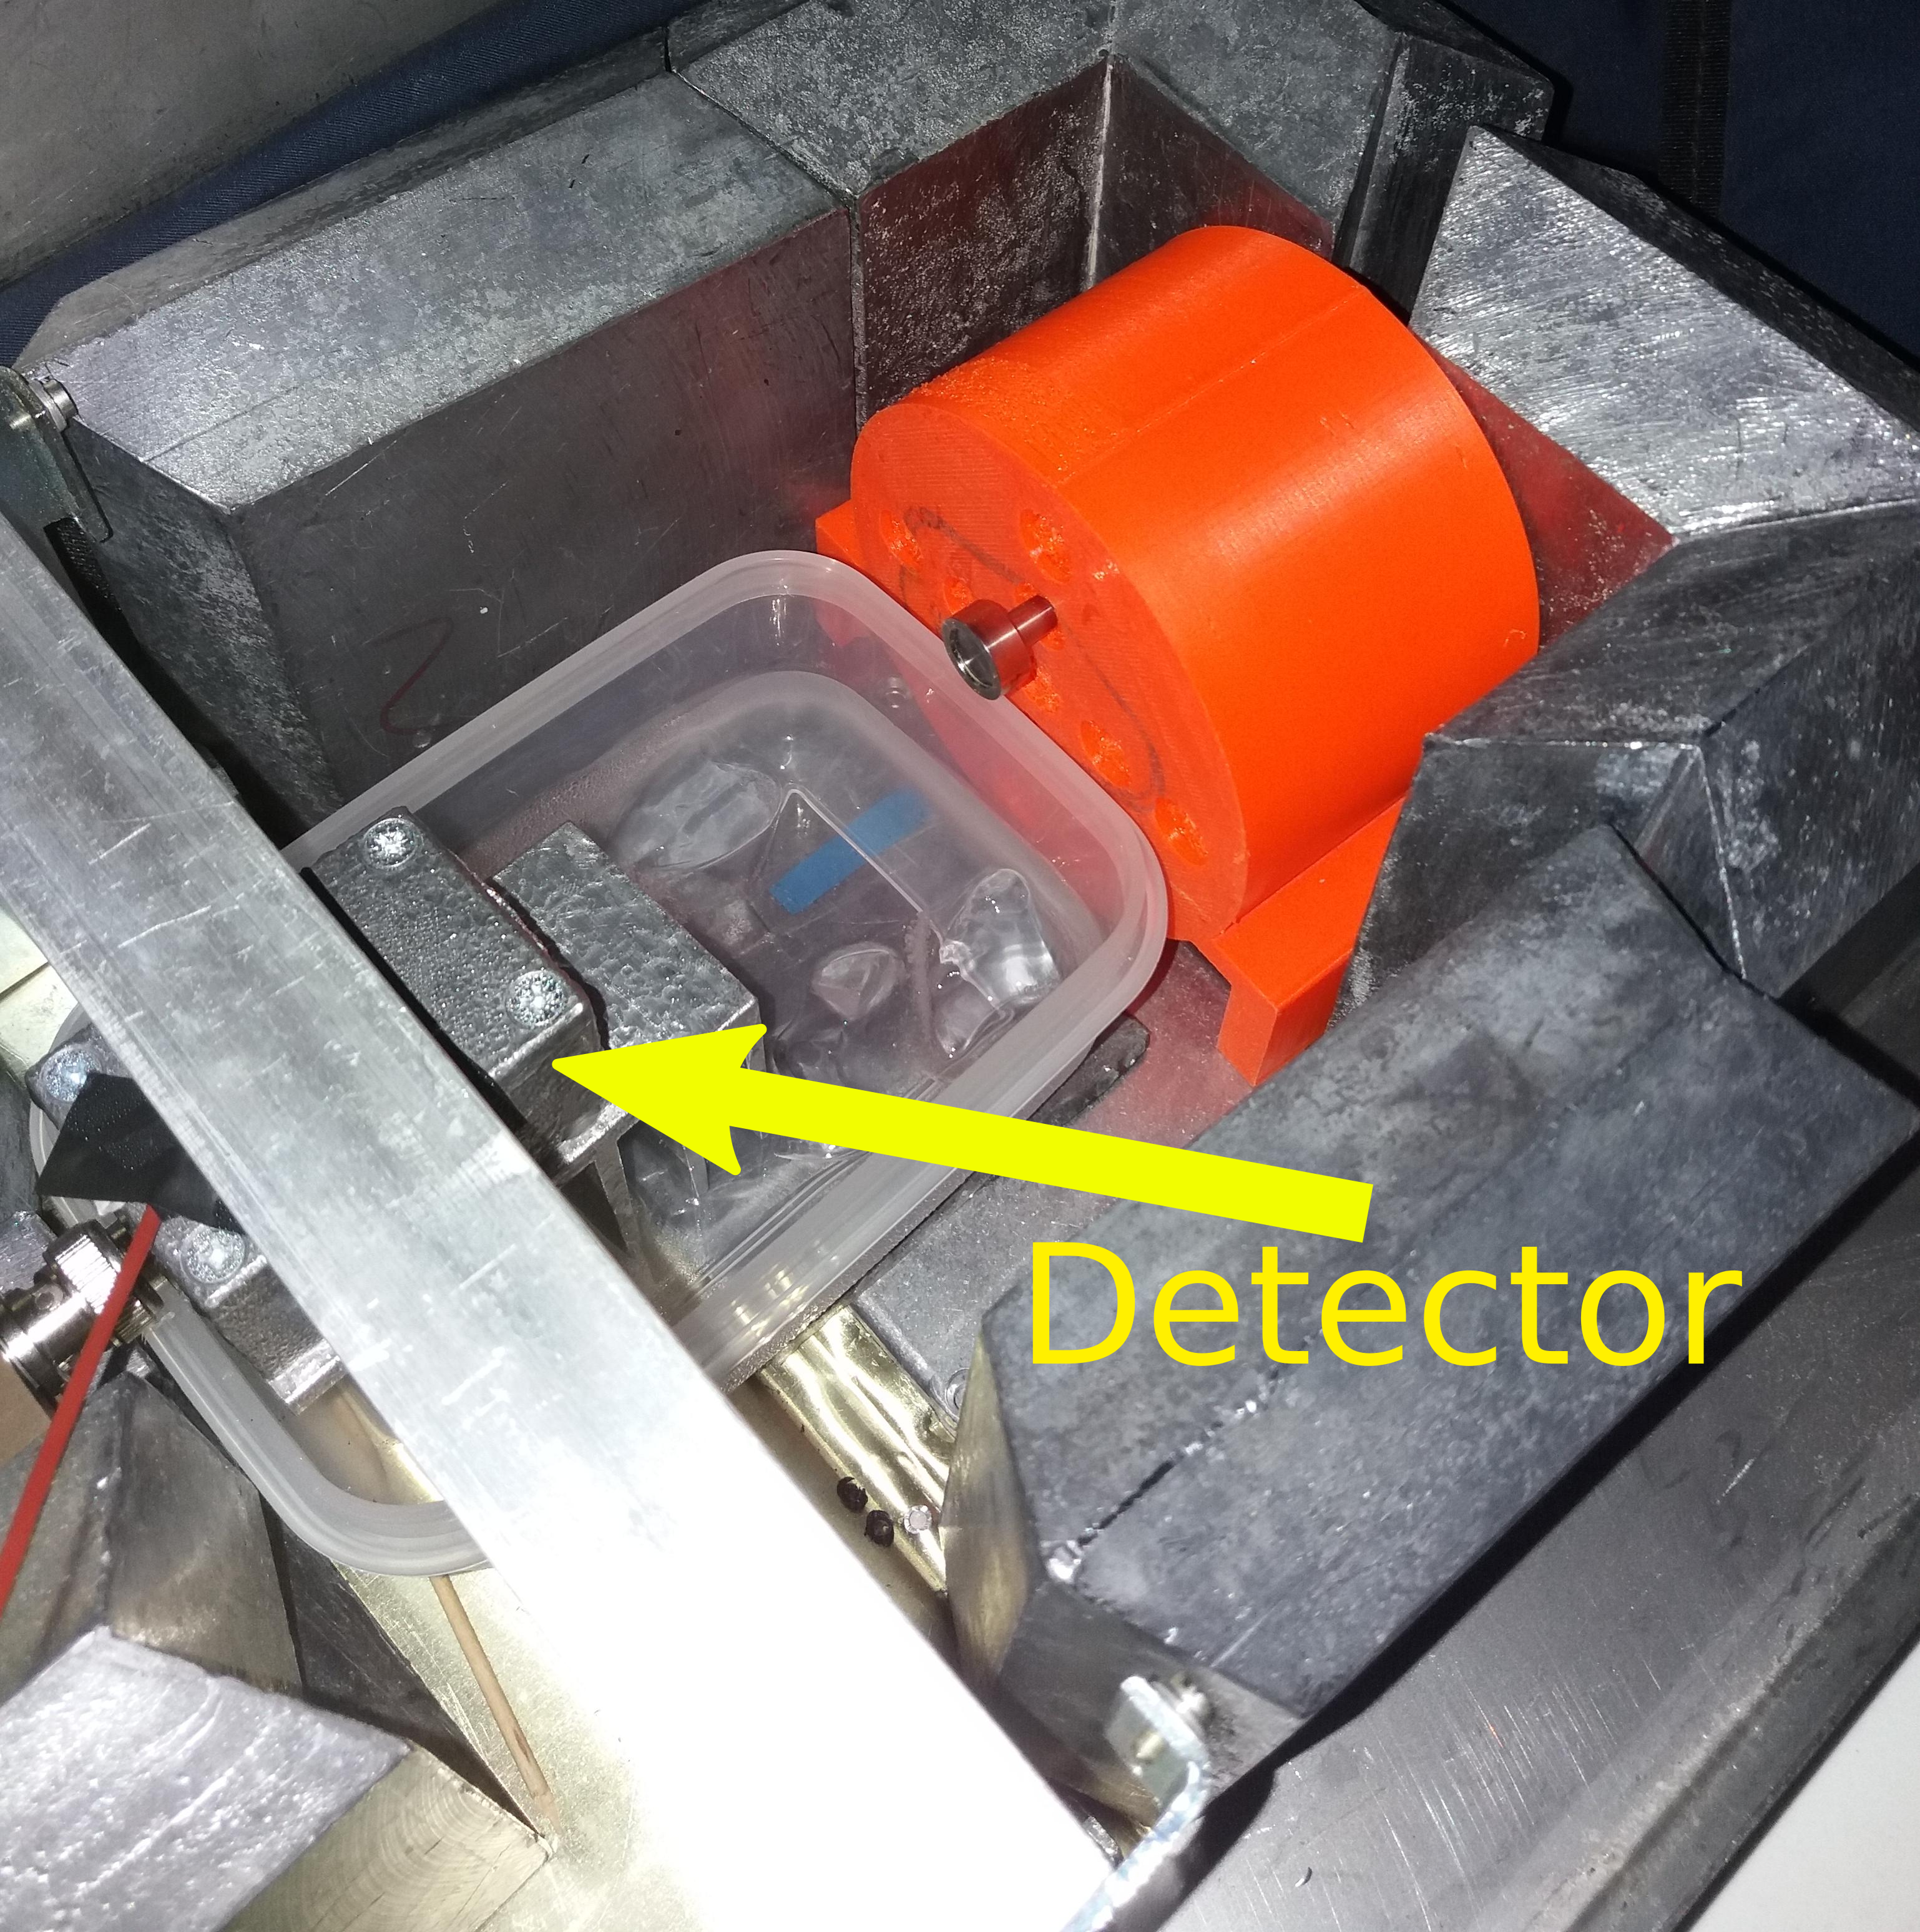
\includegraphics[scale=0.09, angle = 0]{./pictures/chlazeniLedem.png}
 \caption{Detector cooled by ice.}
 \label{cooler}
 
\end{figure}



\begin{figure}[H]
 \centering
 \includegraphics[scale=0.13, angle = 0]{./pictures/TempDiff.png}
 \caption{Measured $^{57}$Co spectra at two different temperatures.}
 \label{coolspectr}
 
\end{figure}
\par
The results show that cooling improves SNR, but its effect is small compared to the effect of proper shielding. The cooling is not used in the following tests on the ORTEC setup.


\section{Test measurement of the $^{57}$Co spectra}
The spectra for each photodiode were acquired for 30 min of live time - MCA allows dead time compensation which extends the total real time of the spectrum acquisition. The source was placed at a distance of 1 cm from the front shielding box (figure \ref{setup}) and to recognise the corresponding peaks, the set of the following filters was placed between the source and the detector:
%The spectra for each photodiode were taken for 30 min of live time - MCA allows dead time compensation, which extends the total real time of spectra acquisition. The source was placed into distance 1 cm from the front shielding crate (figure \ref{setup}) and to recognize the corresponding peaks, the set of the following filters were placed between source and detector:
\begin{itemize}
\item Pb filter: everything should be attenuated.
\item Cu filter: transmitted - 122.1 keV, 136.5 keV absorbed - 14.4 keV, 6.4 keV.
\item Al filter: transmitted - 122.1 keV, 136.5 keV, 14.4 keV absorbed - 6.4 keV.
\end{itemize}



\begin{figure}[H]
 \centering
 \includegraphics[scale=0.09, angle = 0]{./pictures/ORTECsetup.jpg}
 \caption{Setup for $^{57}$Co gamma spectrum measurement with filters. PIN photodiode  is situated inside the shielding crate, which is connected to the preamplifier.}
 \label{setup}
\end{figure}
The spectrum is analysed using our own peak finder program (described in section \ref{search}) to find the characteristic energy components. The 14.4 keV channel position is then used to calibrate the energy axis of the MCA spectrum. The Compton edge caused by the interaction of 122.1 keV photons inside the detector can be expected. The equation \ref{compton} predicts the position to be around 39.5 keV.
%The spectrum is analysed by our own peak finder program (described in section \ref{search}) to find the characteristic energy components. The channel position of 14.4 keV is then used to to calibrate the energy axis of the MCA spectrum. The Compton edge caused by interaction of 122.1 keV photons inside the detector can be expected. The equation \ref{compton} predicts the position to be around 39.5 keV.
\subsection{S14605 test}
The optimal bias voltage of 50 V has been determined experimentally - any further increase does not improve the noise. The measured spectra with no filter, with special filters and only background (fully shielded) are shown in the figure \ref{S14605 spectra}.
%The optimal bias voltage 50 V was deduced experimentally - any further increase does not improve the noise. The measured spectra with no filter, with particular filters and only background (fully shielded) are in the figure \ref{S14605 spectra}.


\begin{figure}[H]
 \centering
 \includegraphics[scale=0.125, angle = 0]{./pictures/S14GammaTest.png}
 \caption{S14605 spectra with founded energy peaks (green lines) and predicted Compton edge (red line).}
 \label{S14605 spectra}
 
\end{figure}


\par
The first peak was determined to be a 14.4 full energy peak as it is absorbed by the Cu filter. The 21.9 keV peak is from characteristic X-rays of the rhodium matrix, and 59.4 keV may also originate from the source matrix. The 67.5 keV and 85.3 keV peaks are most likely characteristic X-rays from the lead shielding. The last two peaks (123.0 keV, 137.7 keV) are from $^{57}$Co. It can be seen that the detection efficiency of the full energy at higher energies (122.1 keV) is very low, and that Compton scattering is preferred interaction effect inside the detector at these energies, resulting in the expected Compton edge. The expected peak at 6.4 keV is hidden in the electronic noise.
%The first peak was determined as 14.4 full energy peak, because the Cu filter absorbs it. The 21.9 keV peak originates from characteristic x-rays of rhodium matrice and 59.4 keV also possibly originates from the source matrice. The 67.5 keV 85.3 keV peaks are most probably characteristic x-ray photons of lead shielding. The last two peaks (123.0 keV, 137.7 keV) are from $^{57}$Co. It can be seen that the full energy detection efficiency of higher energies (122.1 keV) is very small and that the Compton scattering is preferred interaction effect inside detector at these energies, which results into expected Compton edge. The expected peak of 6.4 keV is hidden in the electronic noise.

\subsection{BPW34 test}
The instrumentation was similar to before, but BPW34 had to be operated at a lower bias voltage, so 20 V was chosen as the optimum. The measured spectra are shown in the figure \ref{BPW34 spectra}.
%The instrumentation was similar as before, but BPW34 had to be operated at lower bias voltage and thus 20 V was chosen as an optimum. Measured spectra are in the figure \ref{BPW34 spectra}.

\begin{figure}[H]
 \centering
 \includegraphics[scale=0.125, angle = 0]{./pictures/BPW34GammaTest.png}
  \caption{BPW34 spectra with founded energy peaks (green lines) and predicted Compton edge (red line).}
 \label{BPW34 spectra}
 
\end{figure}
The measured spectra of BPW34 are very similar to the previous one, but the peak heights are about 25 times lower. The results also confirm the fact that the Si semiconductor structure with p-n or p-i-n junction detects the gamma photons with the same signal strength without any dependence on the dimensions. Only the detection efficiency depends on the dimensions.
%The measured spectra of BPW34 is very similar to the previous one, however the peak's heights are approximately 25 times lower. The results also confirm the fact that the Si semiconductor structure with p-n or p-i-n junction detects the gamma photons with the same signal strength without any dependency on the dimensions. Only the detection efficiency is dependent on the dimensions.
\subsection{OPF430 test}
The OPF430 was operated at 20 V. There was a problem with the very low detection efficiency, so the source had to be placed in the shielding box just before the photodiode. Spectra acquired in this way are shown in the figure \ref{OPF430 spectra}.
%OPF430 was operated at 20 V. There was a problem with the very low detection efficiency, so the source had to be put into the shielding box right before the photodiode. Spectra acquired this way are in the figure \ref{OPF430 spectra}.

\begin{figure}[H]
 \centering
 \includegraphics[scale=0.125, angle = 0]{./pictures/OPF430GammaTest.png}
 \caption{OPF430 spectra with founded energy peaks (green lines) and predicted Compton edge (red line).}
 \label{OPF430 spectra}
 
\end{figure}
It can be seen that the count rates are still much lower compared to previous photodiodes. This is probably due to the fact that the detector area is very small. The conclusion is that the OPF430 is capable of capturing the low energy gamma rays, but the efficiency is so bad that it is unusable for any real gamma spectroscopy application.
%It can be seen that the count rates are still much lower in comparison with previous photodiodes. This is probably due to the fact, that the surface of detector is very small. The conclusion is that OPF430 is capable of capturing the low-energy gamma rays, however, the efficiency is so bad that it makes it unusable for any real gamma spectroscopy application.


\chapter{Design of integrated amplifier}
The only way to improve the performance of the spectrometric chain is to integrate the amplification part and a shaper into a small PCB - short the signal routes, reduce parasitic capacitances at preamplifier input and improve the shielding. The various prototypes were designed as double-sided PCBs and manufactured by using the milling machine for PCB to remove cooper from cuprextit plates. The PCB consisting mainly of surface mount deposition (SMD) parts was then assembled by manual soldering.

\section{Scheme and layout}
The main parts of spectrometric chain integrated PCB are: photodiode input connector, preamplifier, second stage amplifier, shaper module, output buffer optimized for 50\nobreakspace$\Omega$ transmission line, bipolar voltage supply for modules and bias voltage supply for photodiode. To surround the sensitive parts with sufficient shielding, the PCB is placed into aluminium box with drilled photodiode window. The full schematic of the integrated amplifier can be seen in the Fig. \ref{schematic} and the real layout for PCB can be seen in the Figures \ref{layout top} and \ref{layout bottom}.



\begin{figure}[H]
 \centering
 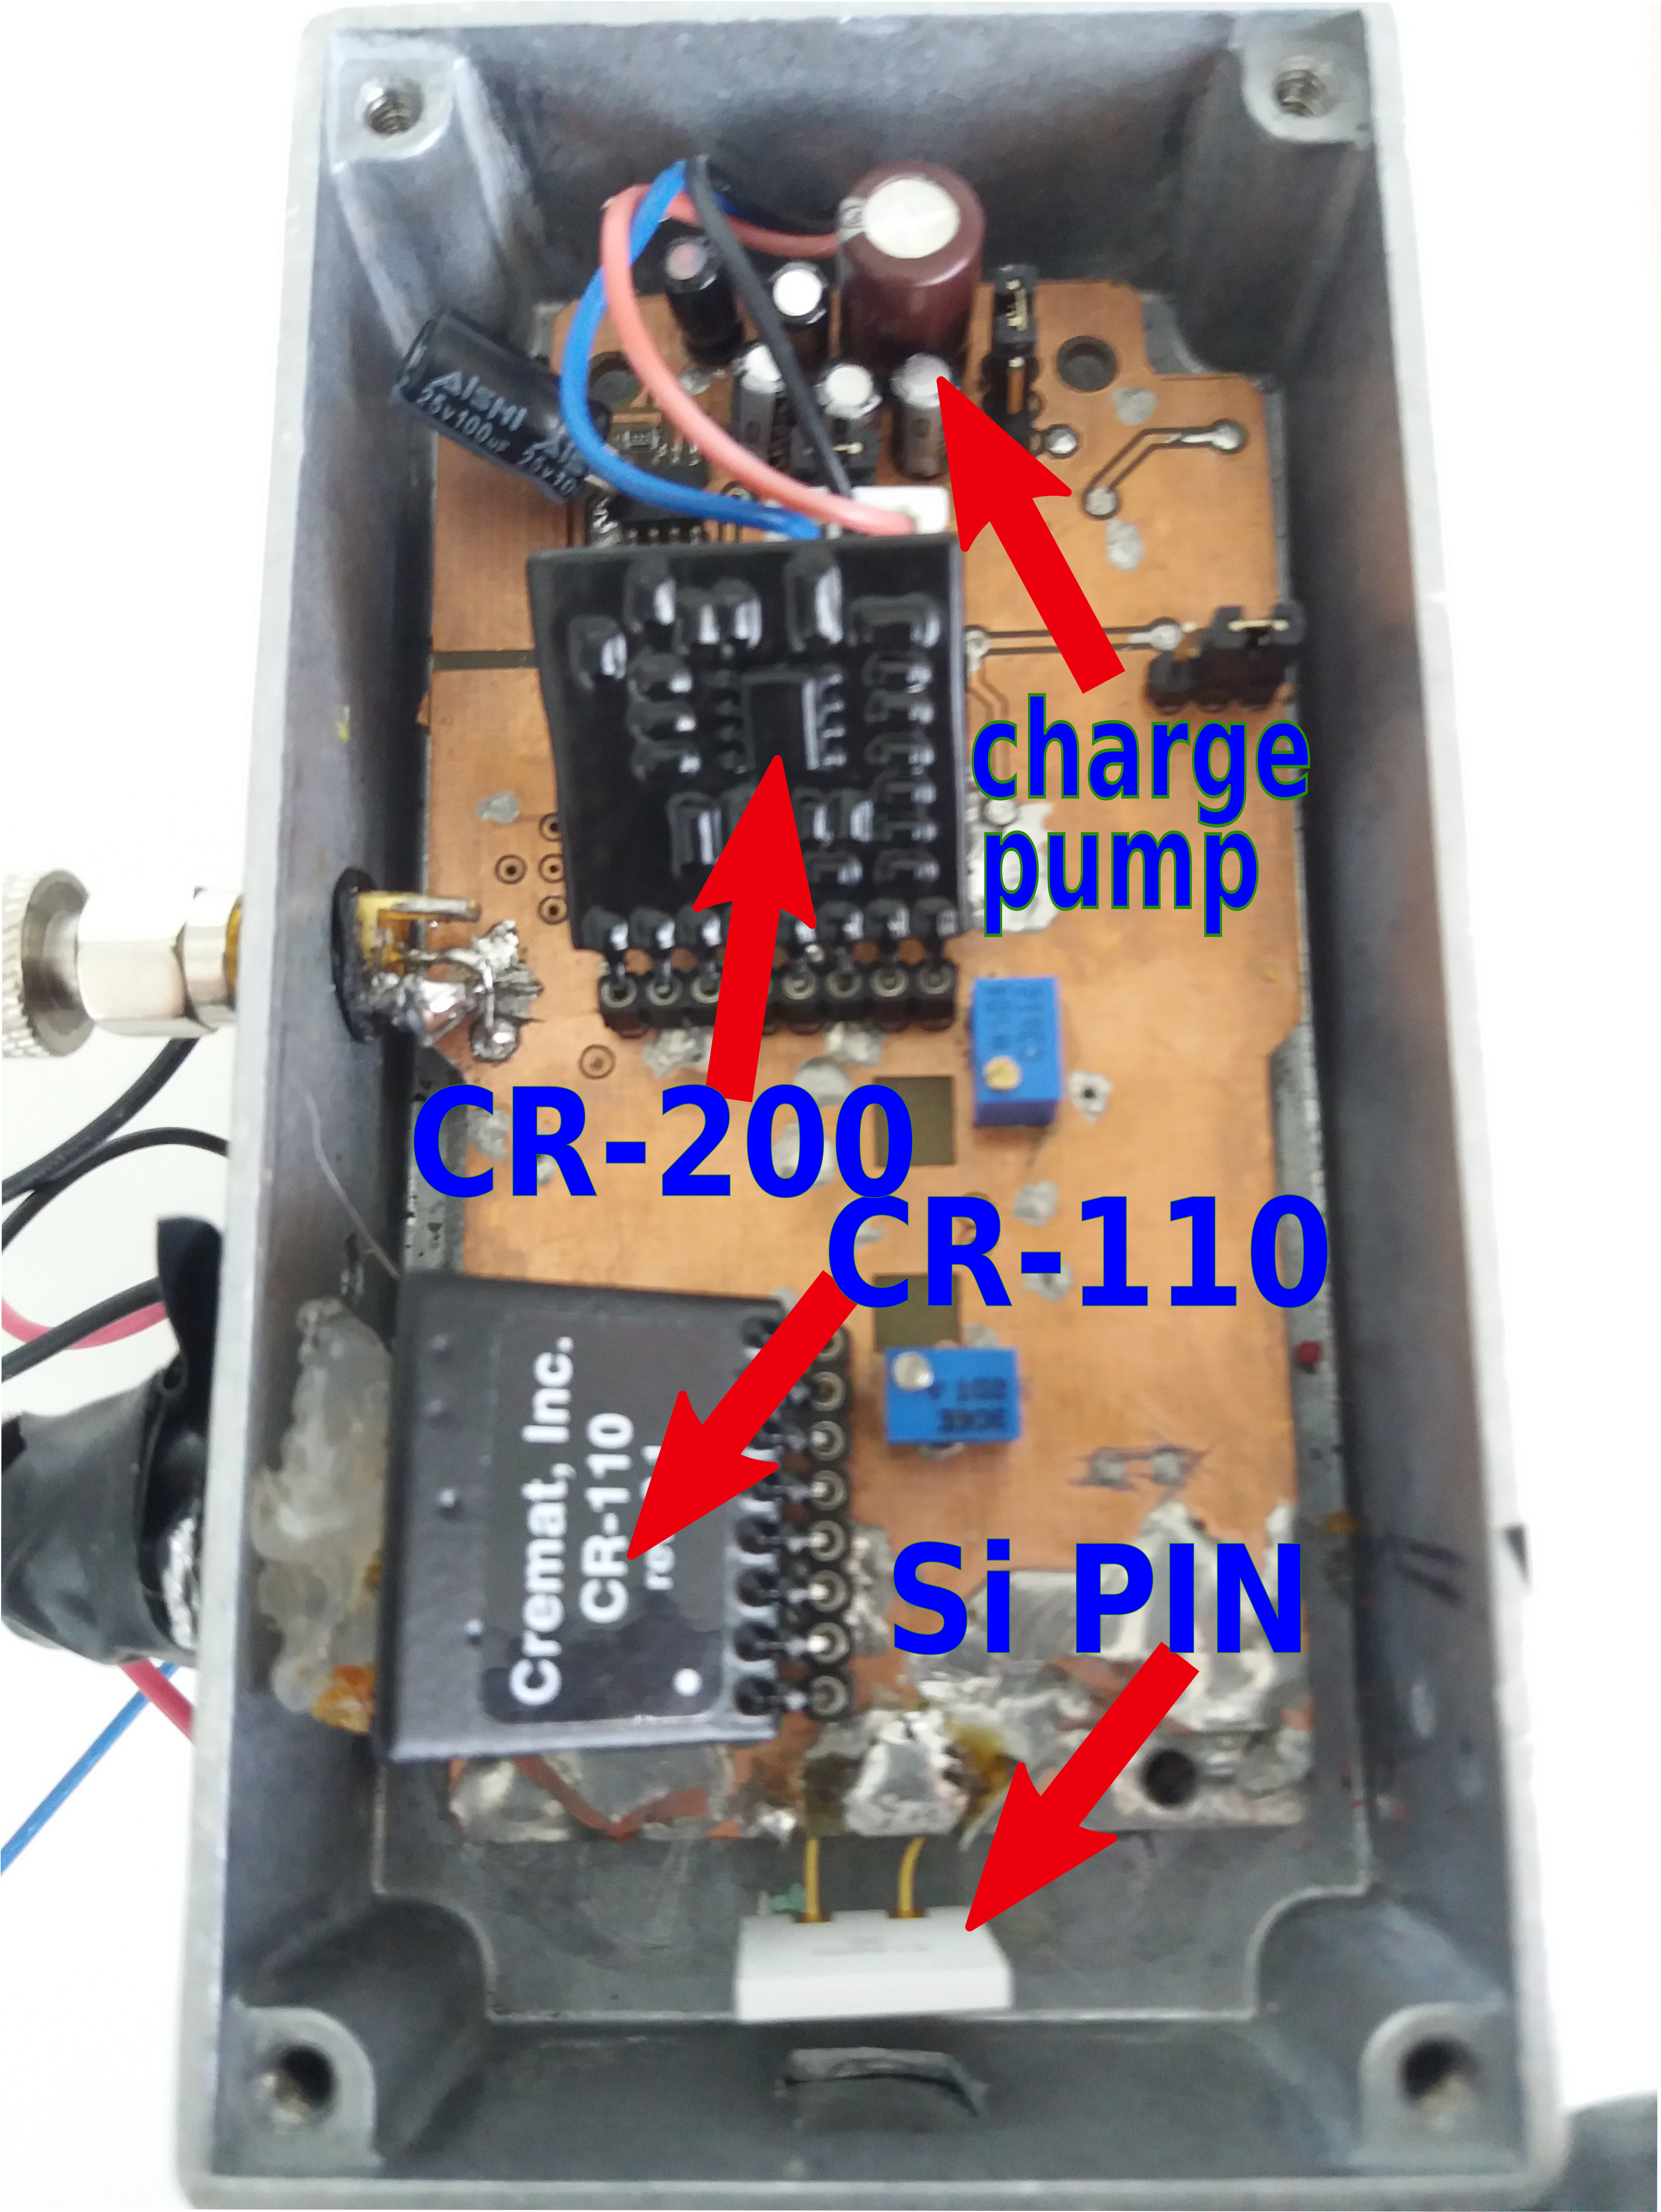
\includegraphics[scale=0.1, angle = 0]{./pictures/SemiInCrateInside.png}
 \caption{Fully assembled PCB with attached cremat modules inside the shielding box.}
 \label{PCBbox}
 
\end{figure}


\begin{figure}[H]
 \centering
 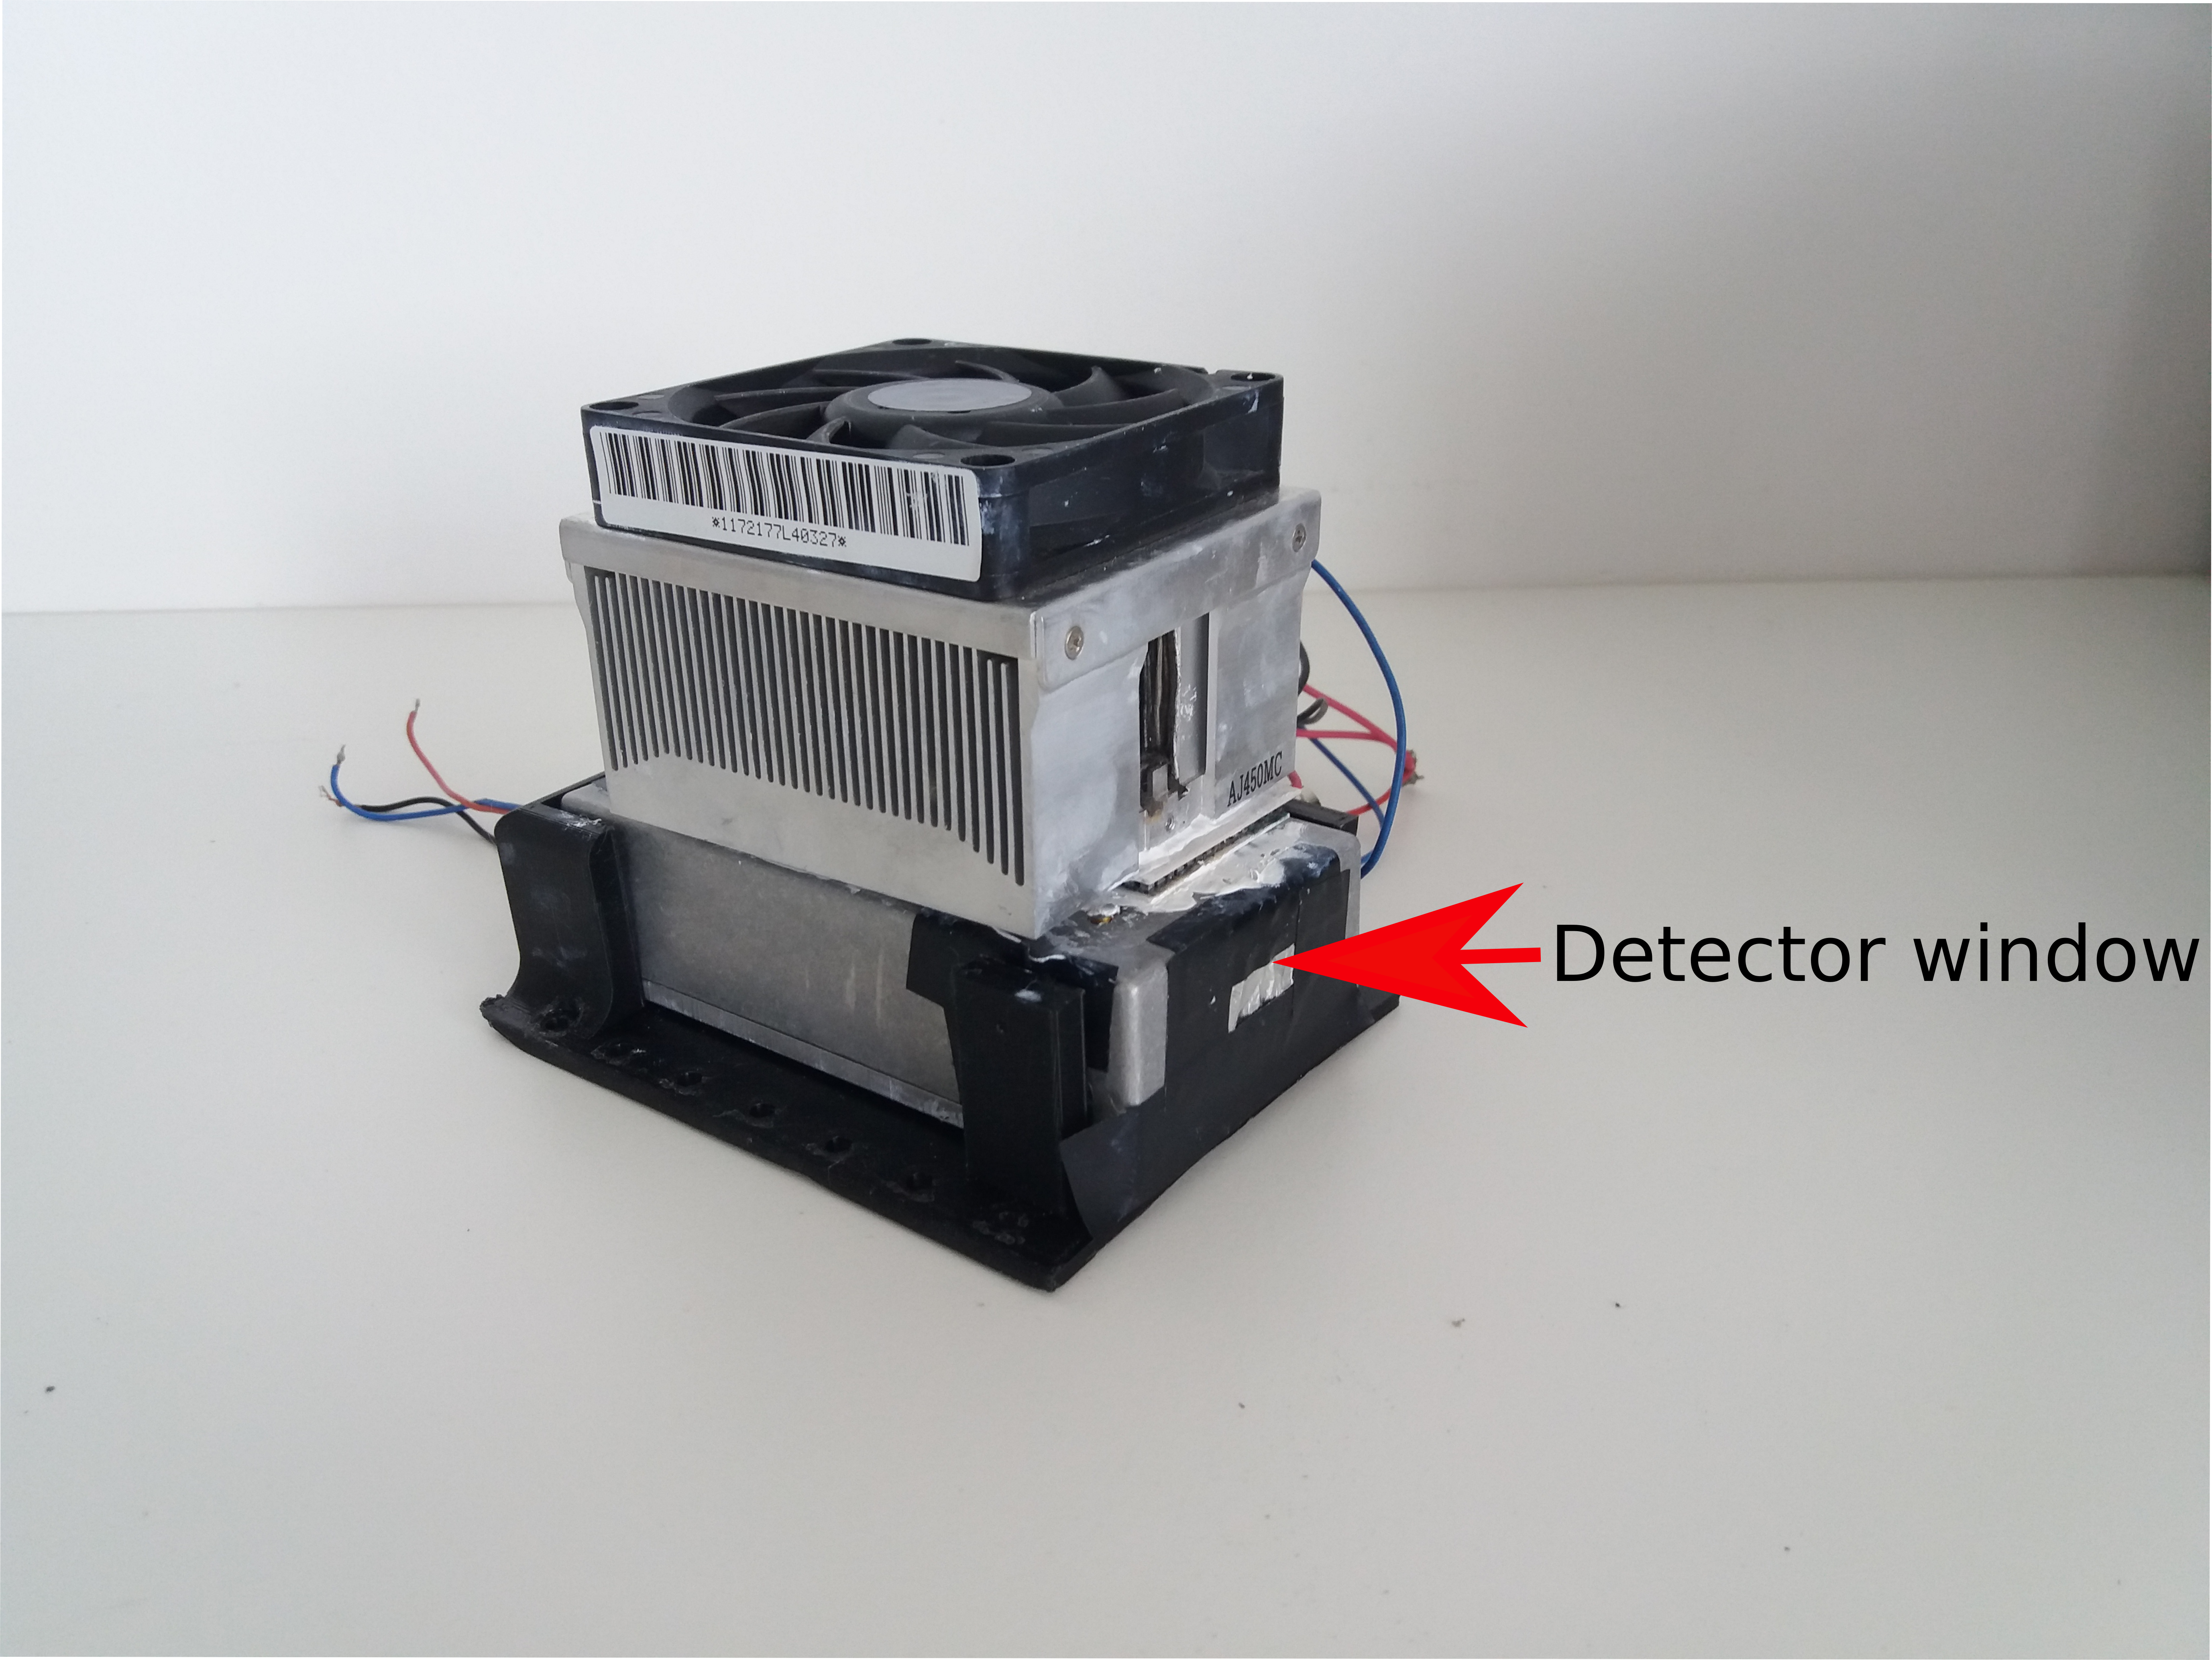
\includegraphics[scale=0.1, angle = 0]{./pictures/SemiInCrate.png}
 \caption{PCB in aluminium box with attached peltier coolers.}
 \label{PCBphyss}
 
\end{figure}



\newpage

\begin{figure}[H]
 \centering
 \includegraphics[scale=0.5, angle = 90]{./pictures/schemaPopis.png}
 \caption{Schematic of spectrometric chain PCB designed in EAGLE \cite{eagle}. Full schematic can be found in attachments.}
 \label{schematic}
 
\end{figure}

\newpage

\begin{figure}[H]
 \centering
 \includegraphics[scale=0.8, angle = 90]{./pictures/S14topLay.png}
 \caption{Layout of spectrometric chain PCB designed in EAGLE \cite{eagle}, top side layer.}
 \label{layout top}
 
\end{figure}

\begin{figure}[H]
 \centering
 \includegraphics[scale=0.8, angle = 90]{./pictures/S14bottomLay.png}
 \caption{Layout of spectrometric chain PCB designed in EAGLE \cite{eagle}, bottom side layer.}
 \label{layout bottom}
 
\end{figure}
\newpage





\section{Grounding and Shielding}
To allow all the currents to have their return path with a sufficient conductivity, the main GND signal has to be spilled all around the circuit board. Even a small resistances in these paths may cause additional noise in signals. Currents from non-signal parts such as charge pump should have their return path different from the path of signal parts, and thus the spilled GND has to be cut to several separate parts connected together only at input voltage connector. This kind of layout is reffered as a star ground structure \cite{star}.

\par
The shielding box has to be connected to GND in carefully selected place to prevent the induced currents from shielding to flow over the signal ground of the detector. The best place to connect the shielding box with GND is near the input voltage connector.


\section{Photodiode input and preamplifier}
The photodiode is situated inside the box, and the cathode is connected to bias voltage and to preamplifier (CR-110) by capacitive coupling (10 nF capacitor). CR-110 application note also mentions an optional 220 $\Omega$ resistor connected before coupling capacitor to prevent CR-110 breakdown by large current spikes. Our experiences show that this resistor should not be omitted.

\par
The signal route has to be as short as possible. The layout should also be designed in ways to reduce the parasitic capacitances at the preamplifier input - the cooper connected to ground (GND) should be removed from areas around the signal input route and around input bias voltage route. 

\section{Amplification}
The preamplifier output is routed over capacitive coupling (to eliminate unwanted offset) and over potentiometer divider (to adjust signal amplitude) to the amplification stages. 

First amplification is achieved by two non-inverting amplifiers with OPA847 opamps. Each stage has the amplification of 32$\times$ (or less, this is different for every of our prototypes). Additional amplification 10$\times$ is done by shaper module CR-220. The OPA847 opamp datasheet \cite{OPA847} describes that these fast opamps are prone to unwanted oscillations, and therefore the GND around the opamp must be removed from both sides of the PCB. The output of shaper module is routed directly to output buffer opamp Max4201. The end of chain is buffered and connected to the output SMA connector mounted onto the aluminium box.


\section{Voltage supply}
The regulation of power supply (usually +15 V and -15 V) is done by LM317 and LM337 regulators, which convert input supply voltages into +7 V and -4 V. The output voltage of regulators is set by two resistors. However, these regulators produce heat, which negatively affects the SNR, so this heat has to be taken out of the circuit board by the thermal bridge connection to the aluminium box. To stabilize the temperature during the long runs, the shielding case has two additional peltier couples with fan attached onto it.

\par
S14605 requires bias voltage around +50 V, which can be supplied by 3-stage charge pump, assembled simply from capacitors, diodes and PWM generator - for example NE555. The charge pump is theoretically designed to multiply the the input voltage +15 V to +60 V. However, due to the fact that the rectifying diodes have some dropout and also   because the charge pump is not a stiff voltage source (even a small currents cause large dropout), the real bias voltage is around +50 V. The pump's output has to be filtered, because it can contain voltage spikes from switching frequency (NE555's frequency is set to 10 kHz). To filter this high voltage output the high-voltage opamp OPA454 is connected as buffer - the pump's voltage is connected as opamp supply, and the voltage from regulator (+7 V) is connected into opamp negative input pin. There is also a jumper which allows to switch between +15 V (for BPW34 photodiode) and +50 V.



\chapter{$^{57}$Co MCA measurement with integrated amplifier} 
In order to properly test the assembled integrated amplifier with attached S14605 photodiode (hereafter referred to as Si PIN detector) and to compare its detection efficiency for 14.4 keV photons with the detection efficiency of the other types of detectors - scintillator and gas detectors - the measurement setup was constructed with a carefully designed geometry.
\par
The on-board gain is set to observe the 14.4 keV energy peak in the second half of the channel range, which on the other hand means that the photons of higher energies cannot be observed as they are in saturation, but the detection of these energies is not our focus.
\par
For each detector the sequence of five measurements was performed - without filter, with three filters and without source. The relative detection efficiency for 14.4 keV is determined by a Gaussian fit of the 14.4 keV peak in spectra with background subtracted. Each spectrum measurement was performed with 1200 s of live time, i.e. with compensation for dead time. 
%To properly test the assembled integrated amplifier with attached S14605 photodiode (further referred as Si PIN detector) and to compare its detection efficiency for 14.4 keV photons with the detection efficiency of the other types of detectors - scintillator and gaseous detectors, the measurement setup with carefully designed geometry was constructed.
%\par
%The onboard amplification is set in a way to observe 14.4 keV energy peak in the second half of the channel range, which on the other hand results into the fact, that the photons of higher energies cannot be observed since they are in saturation, but the detection of these energies is not our focus.
%\par
%For every detector, the sequence of five measurement was performed - without filter, with three filters and without a source. The relative detection efficiency for 14.4 keV is determined by Gaussian fit of the 14.4 keV peak in spectra with subtracted background. Every measurement of spectra ran 1200 s of live time, i.e. with compensation of dead time. 



\section{Measurement setup}
The measurement setup consists of 3D printed parts - plastic holders for each detector and holders for radiation filters. All the holders have to be modular and easily interchangeable to keep the geometry the same for each detector.
The $^{57}$Co source (date of production: 12.10. 2020) is mounted on the transducer (switched off for this measurement). To compare the detection efficiency of detectors with different detection areas, the irradiation has to be done through a collimator, so the detector is irradiated through a hole ($d = 4$ mm) in a lead shielding.
\par
The detector output is connected directly to the ORTEC MCA. For peak identification three filters were placed in front of the lead collimator - Cu (255 $\mu$m), Al (780 $\mu$m), Pb (5 mm).
%The measurement setup consist of 3D printed parts - plastic holders for every detector and holders for radiation filters. All the holders have to be modular and easily interchangeable to allow the geometry to be kept same for each detector.
%$^{57}$Co (date of production: 12.10. 2020) source is mounted onto the transducer (switched off in this measurement). To compare the detection efficiency of detectors with different detection area, the irradiation has to be done through a collimator, therefore the detector is irradiated through a hole ($d = 4$ mm) in a lead shielding.
%\par
%The detector output connector is connected directly to the ORTEC MCA. For the peak identification, three filters were placed before lead collimator - Cu (255 $\mu$m), Al (780 $\mu$m), Pb (5 mm).



\begin{figure}[H]
 \centering
 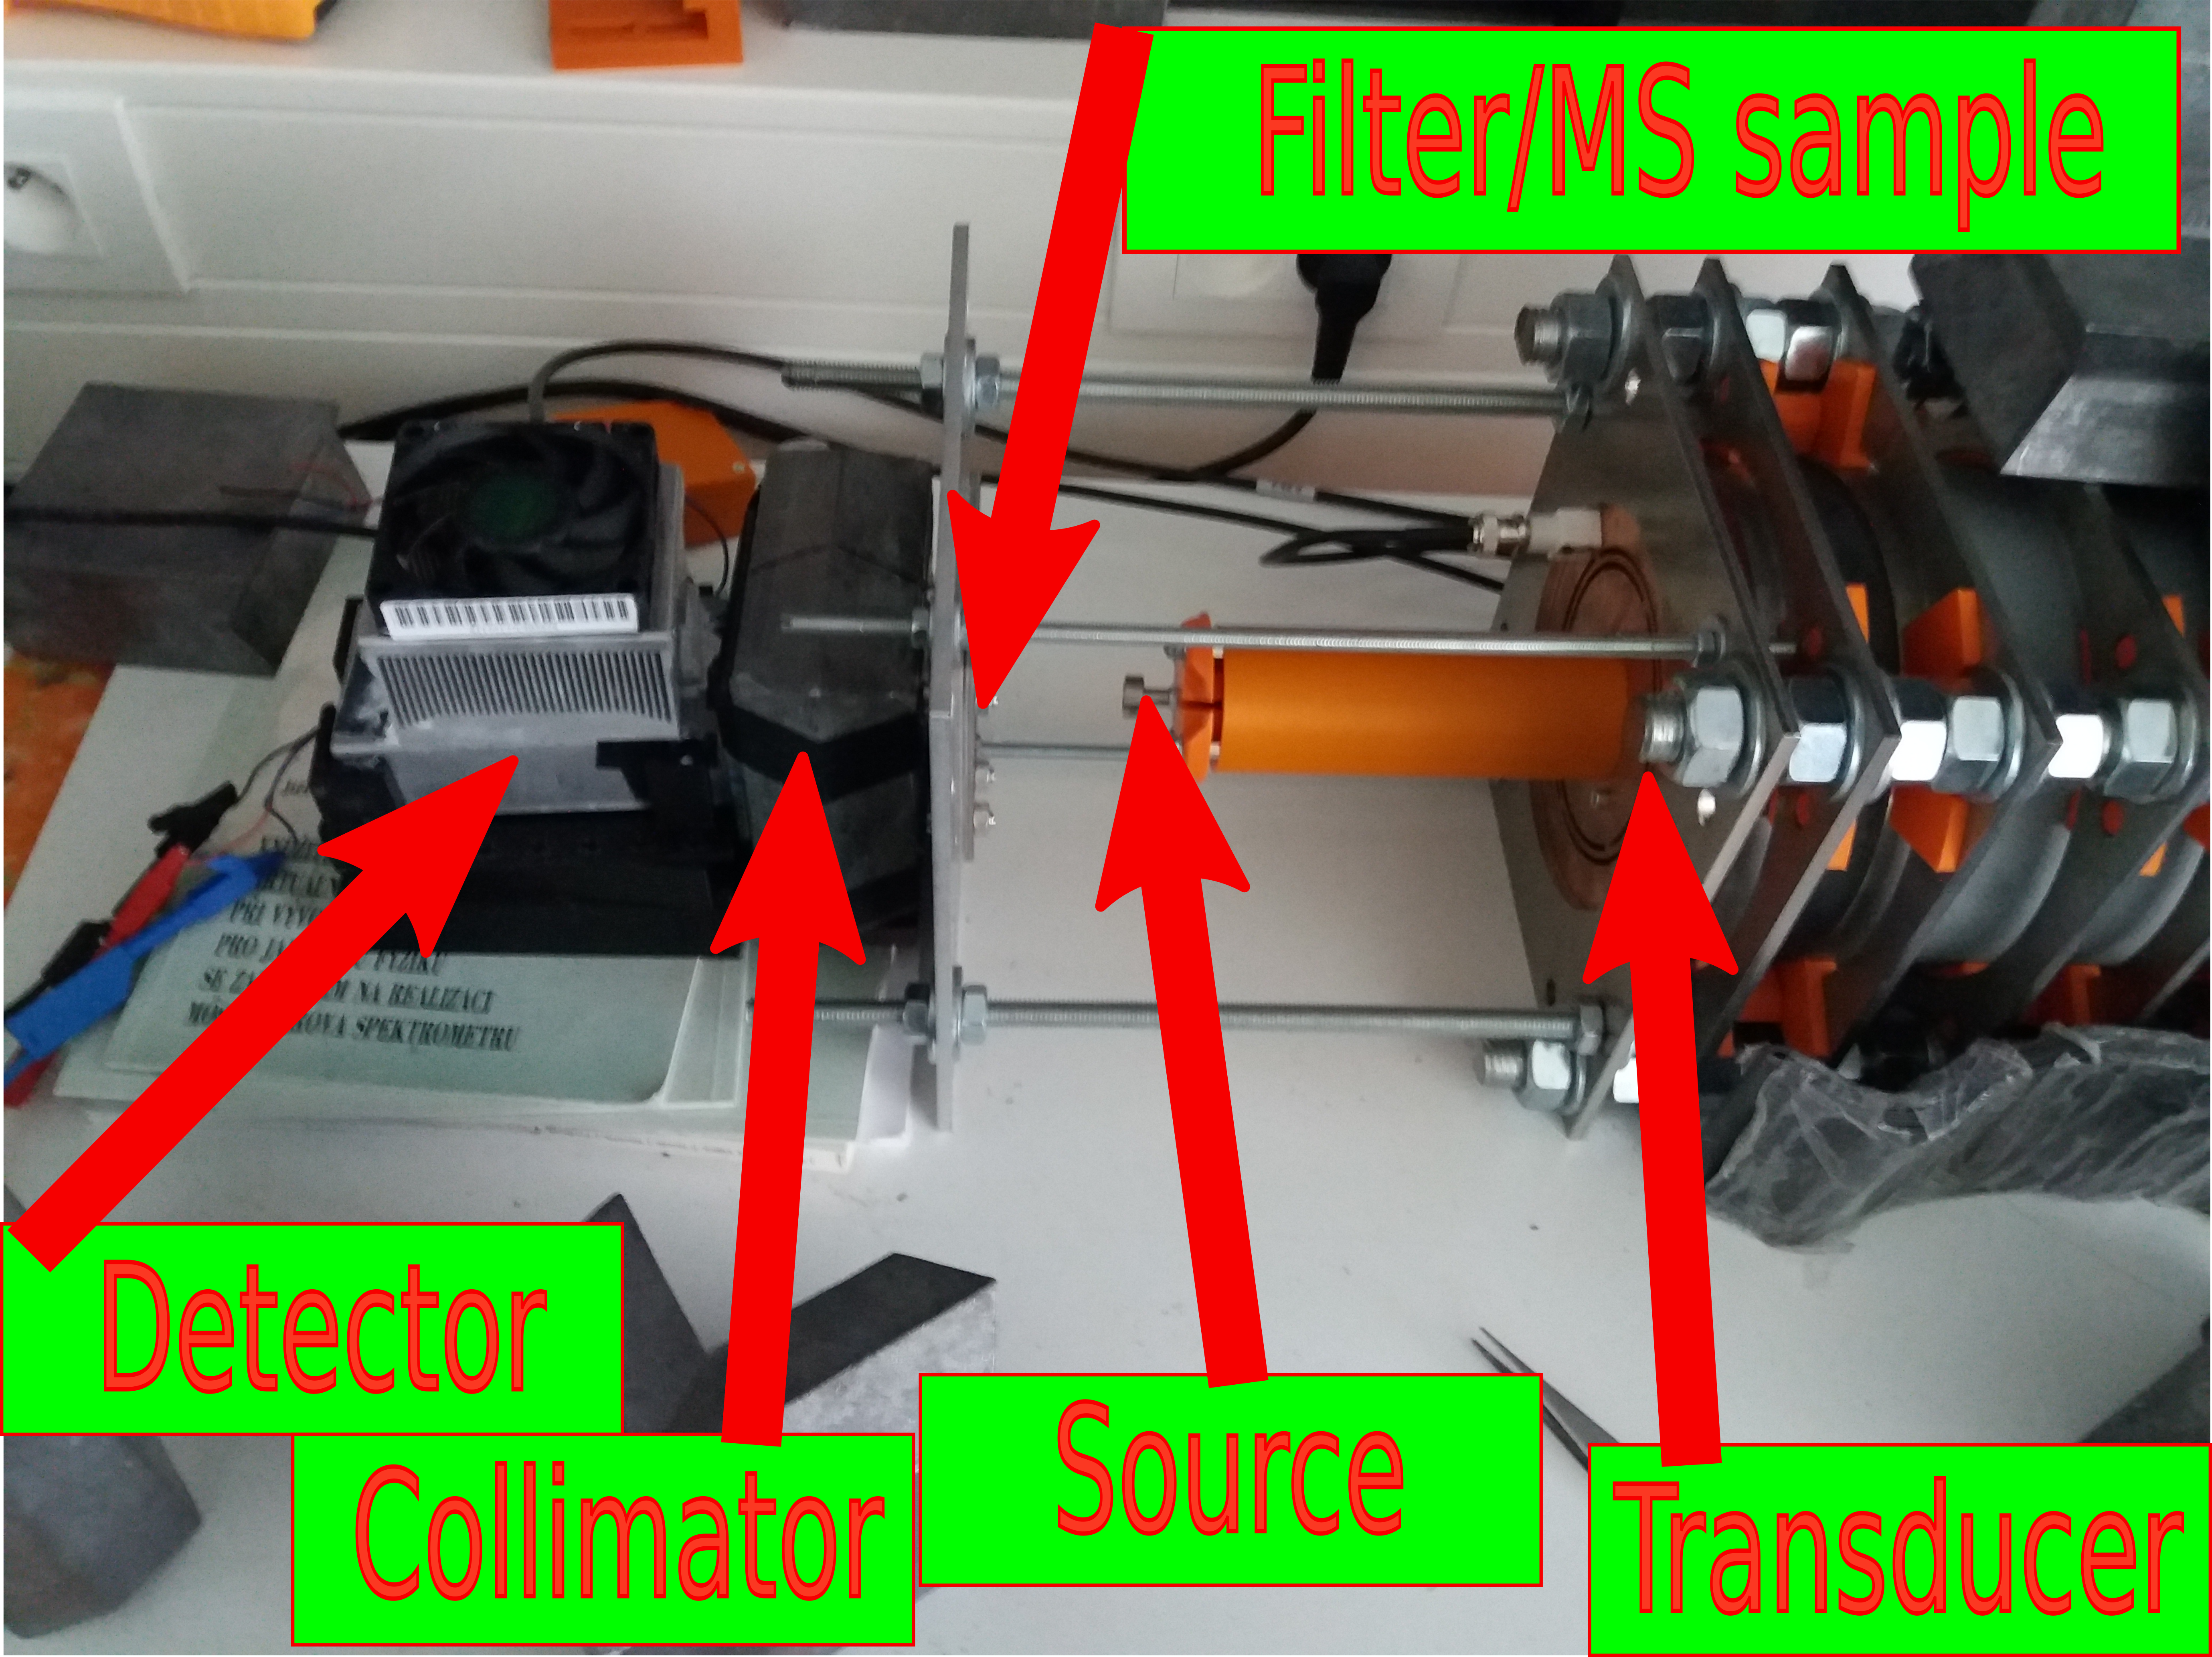
\includegraphics[scale=0.1, angle = 0]{./pictures/TransducerSetup.png}
 \caption{Measurement setup for MCA/MS.}
 \label{meas setup}
 
\end{figure}

\section{Si PIN detector measurement}
The measurement with the Si PIN detector was performed using the previously specified setup. The measured spectra are shown in the figure \ref{Si PIN detector spectra.}.
%The measurement with SI PIN detector was performed by using previously specified setup. The measured spectra are in the figure \ref{Si PIN detector spectra.}.
\begin{figure}[H]
 \centering
 \includegraphics[scale=0.125, angle = 0]{./pictures/SemiSpectre.png}
 \caption{Si PIN detector $^{57}$Co spectra.}
 \label{Si PIN detector spectra.}
\end{figure}
It can be seen that the noise in the spectrum is much lower than in the case of the ORTEC setups. The part of the 6.4 keV peak can also be seen. Several ways have been tried to reduce the noise - cooling with ice, improving the shielding, etc. However, none of them resulted in the peak of 6.4 keV energy without noise. The main part of the remaining noise probably comes from the Si PIN diode capacitance ($C_{\textrm{S14605}} \approx 25$ pF). This was confirmed by using the same PCB with a photodiode of smaller capacitance (e.g. BPW34, $C_{\textrm{BPW34}} \approx 10$ pF). Spectra of the BPW34 connected to the integrated amplifier can be seen in the figure \ref{BPW34 integrated amplifier spectra.}.
%It can be seen, that the noise in spectrum is much lesser than in case of ORTEC setups. The part of 6.4 keV peak can be also seen. Various ways were performed in order to reduce noise - cooling by ice, improving the shielding etc. However, none of them resulted into 6.4 keV energy peak without noise. Main part of remaining noise probably arises from Si PIN diode capacity ($C_{\textrm{S14605}} \approx 25$ pF). This fact was confirmed by using the same PCB with photodiode with smaller capacity (for example BPW34, $C_{\textrm{BPW34}} \approx 10$ pF). Spectra of BPW34 attached to the integrated amplifier can be seen in the figure \ref{BPW34 integrated amplifier spectra.}.


\begin{figure}[H]
\centering
\includegraphics[scale=0.125, angle = 0]{./pictures/BPW34Spectre.png}
\caption{Spectra of BPW34 attached to the integrated amplifier.}
\label{BPW34 integrated amplifier spectra.}

\end{figure}


\section{Scintillator and gas detector measurement}
The same setup was used to measure the relative efficiency of the scintillator and the gas detector. For the gas detector, the LND45479 tube was used, optimised for 14.4 keV detection with amplification electronics also based on Cremat modules. For the scintillator detector, we chose the R6095 photomultiplier tube \cite{R6095} with a C9028-01 socket \cite{C9028}. The scintillator crystal used is YAP(Ce) with a thickness of 0.4 mm and the amplification is done by a custom built amplifier \cite{STEJSKAL2019thesis}. The measured spectra for the scintillator are shown in the figure \ref{Scintillator detector spectra.} and for the gas in the figure \ref{Gas detector spectra.}.
%To measure the scintillator and the gas detector relative efficiency the same setup was used. As a gas detector was used tube LND45479, optimized for the 14.4 keV detection with amplification electronics based also on Cremat modules. In case of scintillator detector, our choice was photomultiplier tube R6095 \cite{R6095} with C9028-01 socket \cite{C9028}. As a scintillator crystal was used 0.4 mm thick YAP(Ce) and the amplification is done by the custom made amplifier \cite{STEJSKAL2019thesis}. The measured spectra for scintillator are in the figure \ref{Scintillator detector spectra.} and for gas in the figure \ref{Gas detector spectra.}.

\begin{figure}[H]
\centering
\includegraphics[scale=0.125, angle = 0]{./pictures/PMTSpectre.png}
\caption{Scintillator $^{57}$Co spectra.}
\label{Scintillator detector spectra.}
\end{figure}
\begin{figure}[H]
\centering
\includegraphics[scale=0.125, angle = 0]{./pictures/GasSpectre.png}
\caption{Gas $^{57}$Co spectra.}
\label{Gas detector spectra.}
\end{figure}
In the spectra of the gas detector, three narrow peaks can be observed - a 14.4 keV peak and two small peaks - 6.4 keV and 19.5 keV. It also has a high level of Compton continuum.
The scintillator sees both the 6.4 keV and 14.4 keV full energy peaks. However, its energy resolution is much worse - both peaks are significantly broader and overlap each other.
%In spectra of gas detector, three narrow peaks can be observed - 14.4 keV peak and two small peaks - 6.4 keV and 19.5 keV. It also has a high level of Compton continuum.
%The scintillator sees both 6.4 keV and 14.4 keV full energy peaks. However, its energy resolution is much worse - both peaks are noticeably wider and they overlap each other. 

\section{Results}
The sum of the total counts for the 14.4 keV and 6.4 keV full energy peaks and the relative detection efficiency with respect to the most effective detector were calculated as follows:
%The sum of total counts for 14.4 keV and 6.4 keV full energy peaks along with the relative detection efficiency with respect to the most effective detector was calculated in the following way:
\begin{enumerate}
\item The spectra with the Cu filter are subtracted from the spectra without the filter. This provides sufficient suppression of the Compton continuum caused by 122.1 keV photons. 
\item The spectra obtained in the previous step are fitted by a sum of Gaussians. The spectra of the Si PIN and the scintillator were fitted by the sum of 2 Gaussians, and in the case of the gas the sum of 3 Gaussians is used due to the wider channel interval.
\item The value of the absolute counts (area under the Gaussian) for the given energy spectra is calculated from the fit parameters with the uncertainties also taken from the fit.
%\item From the spectra without filter is subtracted the spectra with Cu filter. This provides a sufficient elimination of Compton continuum caused by 122.1 keV photons. 
%\item The spectra obtained in previous step is fitted by a sum of Gaussians. Spectra of Si PIN and scintillator were fitted by sum of 2 Gaussians and in case of gas, the sum of 3 Gaussians is used due to the wider channel interval.
%\item The value of absolute counts (area under the Gaussian) for the given energy spectra is calculated from the fit parameters with the uncertainties also taken from the fit.
\end{enumerate}
\begin{table}[H]
\centering
\begin{tabular}{|c|c|c|}
\hline
   & absolute & relative \\ \hline
Si PIN & $143000 \pm 3000$    & $0.291 \pm 0.008$  \\ \hline
gas & $231000 \pm 2000$    & $0.48 \pm  0.01$ \\ \hline
scintillator  & $491000 \pm 9000$    & $1$ \\ \hline
\end{tabular}
\caption{Table of calculated absolute and relative counts of 14.4 keV photons for each detector.}
 \label{144kevEFF}
\end{table}


%The peak of 6.4 keV photons is not fully observable in the case of Si PIN detector. However, a rough estimation can be calculated using parameters obtained from Gaussian fit of partial 6.4 keV peak. Results in table \ref{64kevEFF} are considered to be only indicative. Note also that the setup wasn't designed to detect 6.4 keV photons - some detectors have slices of Al coating in detector window (Si PIN - 1$\times$ 7 $\mu$m thick aluminium foil, scintillator - 3$\times$ 7 $\mu$m thick Al foil, gas - window made of unknown metal). Thick aluminium coating may negatively affect the scintillator detection efficiency.
The peak of 6.4 keV photons is not fully observable in the case of the Si PIN detector. However, a rough estimate can be calculated using parameters obtained from a Gaussian fit of the partial 6.4 keV peak. The results in table \ref{64kevEFF} should be considered as indicative only. Note also that the setup wasn't designed to detect 6.4 keV photons - some detectors have slices of Al coating in the detector window ( Si PIN - 1$\times$ 7 $\mu$m thick aluminium foil, scintillator - 3$\times$ 7 $\mu$m thick Al foil, gas - window of unknown metal). A thick aluminium coating can negatively affect the detection efficiency of the scintillator.

\begin{table}[H]
\centering
\begin{tabular}{|c|c|c|}
\hline
   & absolute & relative \\ \hline
Si PIN & $273000 \pm 8000$    & $1$  \\ \hline
gas & $20000 \pm 4000$    & $0.07 \pm 0.02$ \\ \hline
scintillator  & $184000 \pm 5000$    & $0.68 \pm 0.03$ \\ \hline
\end{tabular}
\caption{Table of calculated absolute and relative counts of 6.4 keV photons for each detector.}
 \label{64kevEFF}
\end{table}


\par
The results in table \ref{144kevEFF} show that the scintillator detector is the best detector for 14.4 keV photons of the three detectors tested. The Si PIN detector does not excel in the detection of these energies and can be classified as the worst of the three. However, from the information provided in the S14605 data sheet \cite{datS14605} we conclude that the efficiency at 6.4 keV energies can be about 51 $\%$ better. This can be partially confirmed by rough estimates in the table \ref{64kevEFF}. To measure the full peak of 6.4 keV photons with the S14605 photodiode, upgrades in the electronics have to be made to increase the SNR, mainly the preamplifier has to be optimised for the capacitance of the S14605.
%The results in table \ref{144kevEFF} show that the scintillator detector is the best detector for 14.4 keV photon among the three detectors that were tested. The Si PIN detector does not excel in detection of these energies and can be classified as the worst of the three. However, by the information provided by S14605 datasheet \cite{datS14605}, we come to a conclusion that the efficiency at 6.4 keV energies can be about 51 $\%$ better. This can be partially confirmed by rough estimations in table \ref{64kevEFF}, which describe the Si PIN as the best detector for 6.4 keV photons. To measure the full peak of 6.4 keV photons with S14605 photodiode, upgrades in electronics have to be made in order to increase the SNR, mainly the preamplifier has to be optimized for S14605's capacitance.





\chapter{Mössbauer spectra measurement}
The previous chapter compared the three detectors in detection efficiency of 14.4 keV photons. This chapter compares them in an efficiency of measuring the MS spectra.
\par
The good detection efficiency of 14.4 keV photons does not necessarily imply the good efficiency of MS spectra measurement and vice versa. Effects, which are not corresponding to the full 14.4 keV photon detection (for example Compton continuum) and generate counts at the channel interval selected for MS measurement, decrease the SNR of MS spectra. To determine this efficiency, setup similar to the one intended for MCA measurement is used again, however, additional parts has to be employed such as a moving transducer and a sample placed into a sample holder. As a sample for this measurement was chosen K$_{3}[$Fe(CN)$_{6}]$, which is characterized by a singlet spectrum.
\par
The entire MS setup is controlled by the special control unit controlled by PC software \cite{STEJSKAL2019thesis}, both developed on DEP. Control unit drives the transducer, regulates its velocity and also processes the incoming pulses from the detector. The control software also takes care of all the data processing and produces MS spectra data files, which are analysed in this chapter.

\par
The detector's output is routed directly to the MS spectrometer control unit, where the channel interval for MS spectra measurement is selected. However, the previous MCA showed that the interval of 14.4 keV peak is different for every detector, so, to compare the detectors in MS efficiency, the channel interval  has to be selected according to the location of 14.4 keV energy peak. We selected this interval as 90$\%$ of FWHM of 14.4 keV energy peak with respect to the results of MCA measurement for each detector.
\par
$^{57}$Co radiation source is mounted onto the moving part of transducer of the "piglet" type also developed on DEP. The transducer is very sensitive to the vibrations and thus it requires to be placed on the soft mat along with the detector and the sample holder. Before the measurement, the velocity calibration routines provided by control SW have to be performed on the transducer to obtain the scaling coefficient which is then used to recalculate the velocity axis from the arbitrary units into the mm$\cdot$s$^{-1}$. 

\par
The three measurements (figures \ref{Si PIN detector MS spectra.}, \ref{Gas detector MS spectra.} and \ref{Scintillator detector MS spectra.}) were performed with the calibrated transducer, one for every detector. One MS spectra was measured for 20 hours including only the valid cycles when the velocity error did not exceed the defined limit.



\begin{figure}[H]
\centering
\includegraphics[scale=0.125, angle = 0]{./pictures/MossSemi.png}
\caption{Si PIN detector K$_{3}[$Fe(CN)$_{6}]$ MS spectra.}
\label{Si PIN detector MS spectra.}

\end{figure}

\begin{figure}[H]
\centering
\includegraphics[scale=0.125, angle = 0]{./pictures/MossGas.png}
\caption{Gas detector K$_{3}[$Fe(CN)$_{6}]$ MS spectra.}
\label{Gas detector MS spectra.}

\end{figure}

\begin{figure}[H]
\centering
\includegraphics[scale=0.125, angle = 0]{./pictures/MossPMT.png}
\caption{Scintillator detector K$_{3}[$Fe(CN)$_{6}]$ MS spectra.}
\label{Scintillator detector MS spectra.}

\end{figure}


Every spectra is fitted by the Lorentzian in the form described by equation \ref{lor}. However, in order to compare the MS parameters between detectors, there was a problem with the different $\Gamma$ in every spectra, which is not caused by the detector, but probably by the transducer. If the SNR$_{\textrm{MS}}$ and $E_{\textrm{MS}}$ (equations \ref{SNR} and \ref{effect}), which both depend on $I$, are to be comparable between the measurements, it is necessary to recalculate the $I$ for every Lorentzian. The recalculation is based on the following consideration: The altered velocity signal can cause the variations in $\Gamma$ of a singlet Lorentzian curve, however, its area $A$ (total number of counts) given by equation \ref{area} should be left unchanged by this effect. So if the $A$ is conserved although the $\Gamma$ is changed, the new amplitudes $I_{\textrm{rec}}$ corresponding to the recalculated Lorentzians with the same $\Gamma_{\textrm{ref}}$  can be obtained by a simple relation $I_{\textrm{rec}} = \frac{\Gamma}{\Gamma_{\textrm{ref}}}I$. As a reference $\Gamma_{\textrm{ref}}$ is taken the smallest $\Gamma$ of the three detectors.
The results obtained for every detector can be seen in table \ref{mossres}.

\begin{table}[H]
\centering
\begin{tabular}{|c|c|c|}
\hline
   & SNR$_{\textrm{MS}}$ & $E_{\textrm{MS}}$ \\ \hline
Si PIN & $27.4 \pm 0.5$    & $0.444 \pm 0.007$  \\ \hline
gas & $35.7 \pm 0.5$    & $0.338 \pm 0.005$ \\ \hline
scintillator  & $54.3 \pm 0.3$    & $0.355 \pm 0.002$ \\ \hline
\end{tabular}
\caption{Measured SNR$_{\textrm{MS}}$ and $E_{\textrm{MS}}$ for every detector.}
 \label{mossres}
\end{table}

The results show that the best SNR$_{\textrm{MS}}$ has the scintillator detector, and thus when it comes to acquiring the MS spectra in transmission geometry, the Si PIN detector is not the best candidate. However, the highest $E_{\textrm{MS}}$ is associated with the Si PIN, and thus it can be employed in some applications where $E_{\textrm{MS}}$ is an important parameter. 









% -----------------------------------------------
% Závěr
% -----------------------------------------------
\chapter*{Discussion}
\addcontentsline{toc}{chapter}{Discussion}
The development of the PIN detector for transmission MS spectroscopy can be continued by using photodiodes with better detection efficiency - by using a Si photodiode with greater thickness or by using a photodiode made of another material with higher $Z$ (e.g. Ge). To fully observe the 6.4 keV energy peak, it will be necessary to use a photodiode with lower capacitance (greater thickness also implies lower capacitance) or a preamplifier with better characteristics. This optimised preamplifier can be realised using discrete opamps. The development can also be continued by mathematical modelling of a better semiconductor detector for MS and by a theoretical simulation of its detection efficiency, using some of the well-known programs for simulating the passage of particles through matter, such as the Geant4 \cite{Geant4}.
\par
The semiconductor detector with a larger detection area can be made up of several PIN photodiodes. However, to reduce noise, each photodiode must have its own preamplifier and amplifier. The final aim is to build a compact Mössbauer spectrometer for backscattering geometry by combining several Si PIN photodiodes with a small transducer in one instrument.
%The development of PIN detector for transmission MS spectroscopy can continue by employing the photodiodes with better detection efficiency - by using Si photodiode with greater thickness or by using a photodiode made of a different material with higher $Z$ (for example Ge). To fully observe 6.4 keV energy peak, it will be necessary to employ a photodiode with lesser capacitance (greater thickness also implies lesser capacitance) or a preamplifier with a better characteristics. The development can also go on by the mathematical modelling of a better semiconductor detector for MS and by a theoretical simulations of its detection efficiency by using some of well-known programs for the simulation of passage of particles through matter such as the Geant4 \cite{Geant4}.
%\par
%The semiconductor detector with greater detection area can be constructed from multiple PIN photodiodes. However, to reduce noise, it is necessary that each photodiode have its own preamplifier and amplifier. Final goal is then to assemble the compact Mössbauer spectrometer for backscattering geometry by combining multiple Si PIN photodiodes and a small transducer into one instrument.


\chapter*{Conclusion}
\addcontentsline{toc}{chapter}{Conclusion}
The first tests of the SI PIN photodiodes were performed on a setup consisting of ORTEC modular parts. All three selected photodiodes (S14605, BPW34 and OPF430) produced spectrometric pulses and the gamma spectra of $^{57}$Co were successfully measured and interpreted. Characteristic full energy peaks of $^{57}$Co (14.4 keV, 122.1 keV and 136.5 keV) were observed, as well as the expected Compton continuum resulting from Compton scattering of 122.1 keV inside the detector. It was found that electromagnetic shielding plays a very important role in noise reduction. The Si PIN photodiodes attached to the charge preamplifier cannot operate properly without sufficient shielding. Cooling the photodiode also had an effect, but it was much less significant.
\par
It was shown that even a cheap Si PIN photodiode (BPW34 and OPF430), originally designed for light detection, could be used as a detector for gamma spectroscopy. However, it has been shown that their detection efficiency is much lower than that of the S14605 photodiode, which is classified as an X-ray detector.
\par
The analog front-end electronics, based on the Cremat preamplifier and shaper, has been successfully developed. It requires only a +15V and -15V power supply to operate. Its output can be connected directly to the MCA. The MS measurement setup using the constructed Si PIN detector was successfully assembled and the transmission MS spectra of a singlet sample were successfully measured.
\par
Two types of measurements were performed to compare the Si PIN detector with the gas and scintillator detector - the 14.4 keV relative detection efficiency measurement and the MS measurement. The only parameter of the Si PIN detector that can be characterised as the best among the detectors tested is the effect of the measurement.
%The first tests of Si PIN photodiodes were performed on setup consisting of ORTEC modular parts. All the three selected photodiodes (S14605, BPW34 and OPF430) produced spectrometric pulses and the gamma spectra of $^{57}$Co were successfully measured and interpreted. Characteristic full energy peaks of $^{57}$Co (14.4 keV, 122.1 keV and 136.5 keV) were observed as well as expected Compton continuum originating from Compton scattering of 122.1 keV inside the detector. It was found out, that the electromagnetic shielding plays a very important role in noise reduction. The Si PIN  photodiodes attached to charge preamplifier can not work properly without sufficient shielding. Cooling the photodiode also had an effect, but its significance was much lower.
%\par
%It was proven, that even a cheap Si PIN photodiode (BPW34 and OPF430) originally intended for detection of light can be employed as detector for gamma spectroscopy. However, it was shown that their detection efficiency is much worse than the detection efficiency of photodiode S14605, which is classified as X-ray detector.
%\par
%The front-end analog electronics based on Cremat preamplifer and shaper was successfully developed. For its functionality it requires only +15 V and -15 V power supply. Its output can be directly routed to the MCA. The MS measurement setup employing constructed Si PIN detector was successfully assembled and the transmission MS spectra of a singlet sample was successfully measured.
%\par
%Two types of measurements were performed in order to compare the Si PIN detector with gaseous and scintillator detector - the measurement of 14.4 keV realative detection efficiency and the MS measurement. The only parameter of the Si PIN detector, which can be characterized as the best among the tested detectors is effect of measurement.



% -----------------------------------------------
% Literatura a prameny
% -----------------------------------------------
%\begin{thebibliography}{99}
%\bibliographystyle{unsrt}
%\nocite{*}
%\bibliography{citations}
%\nocite{MALACARI2020102430}
%\nocite{*}
%\nocite{Tomankova2016_1000061954}
%\nocite{VACULA2021167169}
%\addcontentsline{toc}{chapter}{Literatura}
%\bibitem{gravitation} MISNER, Ch. W.; THORNE, K. S.; WHEELER, J. A. %\emph{Gravitation}. San Francisco: W. Freeman, 1973.
%\end{thebibliography}
%\printbibliography
\printbibliography[notcategory=skipbibliography]
%\newpage
%\chapter*{Attachment: Measurement and analysis programs}
%Measurement folder - scripts for controlling measurement
%\newline
%PulseAnalysis folder - scripts for PMT pulse analysis
%\newline
%FASTanalyze.cpp - calibration data analysis
%\newline
%main.c - Nucleo F446RE's synchronized sampling and PID regulator firmware
\chapter*{List of Symbols and Abbreviations}
\begin{table}[H]
\begin{tabular}{l l}
$\sigma$ & cross section \\
$\sigma_{\textrm{A}}$ & cross section of single atom \\
$F_{\textrm{part}}$ & particle flux \\
$N_{\textrm{s}}$ & average number of particles scattered per unit time from single point target \\
$\Omega$ & solid angle\\
$A$ & area perpendicular to the flux\\
$N_{\textrm{i}}$ & density of interaction centres \\
$N_{\textrm{sc}}(\Omega)$ & average number of particles scattered per unit time multiple interaction centres \\
$N_{\textrm{tot}}$ & average number of particles scattered per unit time multiple interaction centres \\
& integrated over entire solid angle \\
$\delta x$ & material thickness \\
$Z$ & atomic number \\
$I_{\textrm{T}}$ & transmitted radiation intensity\\
$I_{\textrm{0}}$ & incident radiation intensity\\
$\mu$ & total absorption coefficient\\
$N_{\textrm{d}}$ & atomic density \\
$N_{\textrm{a}}$ & Avogadro number \\
$\rho$ & material density \\
$A_{\textrm{w}}$ & molecular weight \\
$f$ & photon frequency \\
$h$ & Planck's constant \\
$\hbar$ & reduced Planck's constant \\
$E_{\textrm{e}}$ & kinetic energy of free electron \\
$E_{\textrm{b}}$ & binding energy of electron \\
$E_{\textrm{2}}$ & scattered photon energy \\
$E_{\textrm{1}}$ & initial photon energy \\
$m_{\textrm{e}}$ & electron mass \\
$M$ & heavy charged particle mass \\
$c$ &  speed of light in vacuum\\
$\frac{dE}{dx}$ &  stopping power\\
$\theta$ &  scattering angle \\
$\varphi$ &  maximum scattering angle \\
$E_{\textrm{c}}$ & energy of electron inside crystal\\
$E_{\textrm{c}}(\vec{k})$ & energy dispersion relation\\
$\vec{k}$ & wave vector \\
$E_{\textrm{g}}$ & energy gap\\
$E_{\textrm{T}}$ & thermal energy\\
$E_{\textrm{s}}$ & electrostatic energy\\
$E_{\textrm{photon}}$ & photon energy\\



\end{tabular}
 \label{symbols}
\end{table}

\newpage
\begin{table}[H]
\begin{tabular}{l l}
$E_{\textrm{F}}$ & Fermi level energy\\
$k$ & Boltzmann constant\\
$\phi$ & electrostatic potential\\
$T$ & thermodynamic temperature \\
$t$ & temperature (Celsius scale)\\
$\omega_{\textrm{photon}}$ & photon angular frequency \\
$E_{\textrm{gamma}}$ & incident gamma photon energy \\
$\epsilon$ & average energy for electron-hole pair generation \\
$n$ & number of generated electron-hole pairs \\
$E$ & energy of incoming particle \\
$F$ & Fano factor \\
$U_{\textrm{R}}$ & reverse voltage \\
$E_{\textrm{0}}$ & base energy level of nucleus\\
$E_{\textrm{M}}$ & pertubed energy level of nucleus\\
$Q_{\textrm{n}}$ & quadrupole momentum of nucleus\\
$m$ & nuclear magnetic number\\
$I_{\textrm{n}}$ & spin of nucleus\\
$E_{\textrm{Q}}$ & energy variation with respect to magnetic quantum number\\
$\gamma$ & gyromagnetic ratio\\
$\delta$ & isomer shift\\
$\mu_{\textrm{m}}$ & magnetic momentum of nucleus\\
$L_{\textrm{v}}$ & Lorentzian in MS spectrum\\
$v$ & relative velocity of radiation source and MS sample \\
$v_0$ & resonant velocity \\
$A$ & area under Lorentzian \\
$\Gamma$ & FWHM of Lorentzian\\
$I_{\textrm{MS}}$ & amplitude of Lorentzian\\
$B$ & MS background level \\
$E_{\textrm{MS}}$ & MS effect of measurement \\
SNR$_{\textrm{MS}}$ & MS signal to noise ratio \\
$Q$ & charge \\
$U$ & voltage \\
$I$ & current \\
$I_{\textrm{G}}$ & FET gate current \\
$I_{\textrm{D}}$ & dark current \\
$C_{\textrm{f}}$ & feedback capacitance \\
$R_{\textrm{f}}$ & feedback resistance \\
$G$ & gain \\
$en_{1}$ & thermal noise of the first stage FET \\
$en_{2}$ & thermal noise caused by feedback resistance \\
$in$ & shot noise \\
$noise$ & total noise \\
$\omega$ & signal angular frequency\\
$j$ & complex unit \\
$g_{\textrm{m}}$ & FET transconductance \\
$\tau$ & decay constant\\
$U_{\textrm{A}}$ & pulse amplitude\\
$C_{\textrm{in}}$ & input capacitance \\
$C_{\textrm{j}}$ & detector capacitance \\

\end{tabular}
 \label{symbols2}
\end{table}


\newpage
\begin{table}[H]
\begin{tabular}{l l}

$C_{\textrm{s}}$ & amplifier input capacitance \\
$d$ & collimator diameter \\
$I_{\textrm{rec}}$ & recalculated amplitude of Lorentzian\\
$I_{\textrm{original}}$ & original amplitude of Lorentzian\\
$\Gamma_{\textrm{ref}}$ & original FWHM of Lorentzian\\
FWHM$_{\textrm{CR-100}}$ & FWHM limit given by CR-110 \\
FWHM$_{14.4}$ & FWHM of the 14.4 keV peak \\
FWHM$_{\textrm{Fano}}$ & FWHM given by fano noise \\


\end{tabular}
 \label{symbols3}
\end{table}


\begin{table}[H]
\begin{tabular}{l l}

PCB & printed circuit board \\
SNR & signal to noise ratio \\
PMT & photomultiplier tube \\
DEP & Department of Experimental Physics \\
MCA & multichannel analyser \\
APD & avalanche photodiode \\
CCD & charge-coupled device\\
CMOS & complementary metal–oxide–semiconductor\\
FWHM & full width at half maximum\\
GND & ground\\
YAP(Ce) & yttrium aluminium perovskite dopped by cerium\\
MS & Mössbauer spectroscopy\\
MPC & model predictive control \\
PID & proportional–integral–derivative\\



\end{tabular}
 \label{shorts}
\end{table}

\chapter*{Appendix}
\section*{Schematic and layout of the integrated amplifier}
Full EAGLE schematic and layout are in the folder IntegratedAmplifier. 


\begin{figure}[H]
 \centering
 \includegraphics[scale=0.38, angle = 90]{./pictures/schemaPopis.png}
 \caption*{Schematic of integrated amplifier.}
 \label{schematic}
 
\end{figure}



\begin{figure}[H]
 \centering
 \includegraphics[scale=0.8, angle = 90]{./pictures/S14topLay.png}
 \caption*{Layout of integrated amplifier, top side layer.}
 \label{layout top}
 
\end{figure}

\begin{figure}[H]
 \centering
 \includegraphics[scale=0.8, angle = 90]{./pictures/S14bottomLay.png}
 \caption*{Layout of integrated amplifier, bottom side layer.}
 \label{layout bottom}
 
\end{figure}

\section*{Peak searching program}
File SpectreAnalyzer.cpp: C++ program for automatic searching of peaks in spectrum.


\end{document}
% Konec souboru %%%%%%%%%%%%%%%%%%%%%%%%%%%%%%%%%%%%%%%%%%%%%%%%%%%%%%%%%%%%
